\documentclass[12pt,a4paper]{article}

\usepackage[utf8]{inputenc}
\usepackage[T1]{fontenc}
\usepackage[english]{babel}
\usepackage{lmodern}
\usepackage{microtype}
\usepackage{geometry}
\usepackage{csquotes}
\usepackage[authoryear,round]{natbib}
\usepackage{float}
\usepackage{hyperref}
\usepackage{booktabs}
\usepackage{array}
\usepackage{enumitem}
\usepackage{xcolor}
\usepackage{amsmath}
\usepackage{amssymb}
\usepackage{graphicx}
\usepackage{pdflscape}
\usepackage{tikz}
\usetikzlibrary{positioning,arrows.meta}
\usepackage{setspace}
\doublespacing

\geometry{left=30mm,right=30mm,top=30mm,bottom=30mm}
\hypersetup{
  colorlinks=true,
  linkcolor=black,
  citecolor=black,
  urlcolor=blue
}
\setlist[itemize]{topsep=4pt,itemsep=2pt}
\setlist[enumerate]{topsep=4pt,itemsep=2pt}

% M&M: tables are numbered with consecutive Roman numerals
\renewcommand{\thetable}{\Roman{table}}

\title{\textbf{Consciousness as Interpretation}\\
\large A Coupling Model of Consciousness}
\author{Babylon Project}
\date{}

\begin{document}
\maketitle
\thispagestyle{empty}

% -----------------------------------------------------------------------
% Abstract
% -----------------------------------------------------------------------
\begin{center}
\textbf{Abstract}
\end{center}
\noindent
Since Descartes wrote \emph{cogito, ergo sum}, accounts of consciousness can
broadly be divided into two positions. Either the body produces conscious
experience, or it receives conscious experience from outside. This paper will
examine the gaps both positions leave and ask if a new approach is able to
eliminate them. In addition to that, the paper will take a closer look at the
two opposing components and their interaction. I will establish a process
between the body and a specified ``outside''. For this I use a timeless relational field instead of
an electromagnetic field. The result will be a model in
which consciousness is a personalized data mapping. The model draws on recent
work in physics and biology. I provide a variety of derivations and simulations to make it more accessible.
These I also use to test its coherence against known medical cases.

\bigskip
\noindent\rule{\linewidth}{0.4pt}
\bigskip

\newpage

% -----------------------------------------------------------------------
\section{Introduction}
\addcontentsline{toc}{section}{Introduction}

Every human being experiences themselves as an individual. Even identical twins in
the same room experience the world as completely different and entirely their own.
Proponents of the production model would say these are small differences in what is
experienced. Proponents of the receiver model would say the difference comes from
outside and is received. Is the answer that simple, and which of the two is right?

This will be our first step in the paper. We discuss what gaps exist in both models
and what we can take away by examining them. To go further ahead and construct new
architecture we look at what we can measure. Much of what shapes our reality can be
pinned down to precise formulas and data. This paper will use the available data and
models to map the boundaries of the ``outside'' and bring it into a clearly described
physical form. This quantum field will act like a data server for us. In addition to
that we will categorize the available local data sources of the body hardware.

Newer scientific tests open an extended view of the possible interaction of the body
and the server. Latest tests are showing that quantum coherence in wet, warm systems
is not ruled out \citep{babcock2024, kalra2023}. This opens up different solution paths without having to rely on
local electromagnetic fields bound to a body. With all the components of our model in
place the paper establishes a process of a personalized data mapping. This represents
our consciousness.

At the end of this paper the model with its established formulas will be applied to
an array of medical cases.

\section{What Must a Model of Consciousness Explain?}
\label{sec:existing_models}

No two people experience the same world in quite the same way. They may stand beside
one another before the same building, listening to the same music as rain begins to
fall, yet each forms a different image. Experience belongs to a particular body,
carries the history of a particular life, and appears from one position at one moment.
Any model of consciousness must explain how a shared world acquires this individual
form.

Two broad answers have organised the debate.

\paragraph{The Production Model.}
On this account, everything needed for consciousness remains within the body. Present
sensory and bodily signals are interpreted through memory, language, learned
categories, expectation, and current physiology. Consciousness results from this
activity, giving biology, learning, and individual difference a clear place. The same
boundary also sets its limit. Every relation in experience must
arrive through present input, remain available in local storage, or be reconstructed
from what is already there.

Contemporary theories describe this local work in different ways. Global neuronal
workspace theory emphasises widespread availability. Integrated information theory
turns to the system's irreducible causal structure, while predictive-processing
accounts describe the continual inference behind perception
\citep{dehaene2011,tononi2004,raoballard1999,friston2010}. They disagree about what
does the decisive work, yet all place it within the physical system. The term
Production Model will refer to this shared boundary rather than to any one of these
theories.

Two problems remain at this boundary. Local memory is finite, and what it retains does
not remain unchanged. It cannot be treated as a complete archive of every relation
that may later enter experience. If a relation is missing from both present input and
local history, a closed producer gives it no route into experience. Even when all the
required data are available, the passage from physical processing to one situated
image is still carried by the phrase that the brain produces it.

\paragraph{The Receiver Model.}
The opposing tradition is older. William James distinguished productive from
transmissive brain function, allowing the brain to shape an individual stream without
generating its wider basis \citep{james1898}. The Receiver Model places that basis
outside the body and treats the brain as receiver or filter. Local memory no longer
sets the limit, but a physical receiver still needs something transmissible, a channel,
and a rule connecting the source to this organism. Reception alone supplies none of
them.

Received content also lacks an individual biography, bodily position, and present
moment. A further process must give it the form in which it is experienced here and
now. The body cannot remain a passive antenna, because a completed consciousness
cannot simply arrive from elsewhere. Reception moves individuation without explaining
it.

The two models begin at opposite ends, but the gaps between them suggest the same
missing operation. A wider basis need not contain a finished consciousness. It might
contain relations that have yet to acquire a viewpoint. The body, in turn, need not
generate the entire data basis. It might contribute the history, present state, and
physical position through which those relations become an individual experience. If
neither side is conscious alone, is their meeting itself the conscious image?

This would be a collaboration rather than a compromise. The wider basis would not
transmit a finished experience, and the local system would not construct one from a
closed store. Each would contribute what the other lacks. The remaining question is
how relations without a viewpoint or local time and a living system can come together
at one place and moment as one individual image.

The Interpreter Model begins with that question. It first considers the living
component, then the wider relational basis, and finally the connection between them.

\section{The Local Client and Its Stored Configuration}
\label{sec:local_client}

Every conscious image belongs to one body. It carries the marks of its history, its
present condition, and the place from which it looks at the world. Wider relations
alone cannot give an image this personal form. So the model begins with the
biological system itself, and we call it the local client: the place where shared
data finally becomes something seen and lived.

\subsection{A lifetime structure and a present state}

What makes an experience belong to one person? Part of the answer is what a life
leaves behind. Development, memory, language, learned categories, habits, and the
slow adaptation of the nervous system all leave a physical structure that changes
only slowly. We write it $B_i$. It is the stored configuration through which incoming
relations take on a familiar form. This is why two people can meet related data and
still form different images: their structures differ, $B_i\not\equiv_K B_j$, as
Equation~\eqref{eq:individuality} states formally.

Yet nobody is quite the same from one moment to the next. Attention, fatigue,
medication, recent activity, and the current state of the body shift a person within
this longer-lived structure, over milliseconds or hours, without replacing who they
are. We write this present position $B_i(t)$. The distinction matters, because it lets
us tell a passing disturbance of the mapping from a lasting, structural loss.

Then there is what arrives right now. Current sensory and bodily input,
$I_{\mathrm{syn}}(t)$, ordinarily anchors where something comes from, where the body
is, and which event is being interpreted. Together these elements make up the local
data side.
\[
  D_i^{\mathrm{local}}
  =\{\text{biological carrier},B_i,B_i(t),I_{\mathrm{syn}}(t)\}.
\]
We keep this separation as the model moves on from the local client to mapping and
physical realisation. All symbols, including those introduced later, are defined in
Table~\ref{tab:notation}.

\subsection{The contribution and limit of local memory}

How much can the body hold on its own? Less than one might think. Memory is not a
recording. It selects, rebuilds what it recalls, stores it again in changed form, and
loses detail over time \citep{schacter2007}. What it keeps is an acquired
configuration, the learned relations and traces that earlier experience has left
behind, not a complete copy of the world.

There is also a hard limit. In the standard random-pattern Hopfield network, a
classic model of associative memory, recall begins to fail at a load of about 0.14
patterns per unit, roughly 14 stored patterns for every 100 units \citep{amit1985}.
A network of fixed size can therefore take in only so much. Beyond that point, new
patterns no longer add memories but disturb the old ones. For any finite network of
$N$ units the critical load is finite as well (Eq.~\eqref{eq:hopfield_finite_load}).

Memory does what it is good at. It gives incoming data a familiar place in a life and
a particular point of view, without having to contain every relation that enters
present experience.

This division can be tested at first contact with something new. If prior exposure,
genotype, endocrine state, familiarity, and the response are measured together, a
response the body was biologically prepared for can be told apart from a learned
pattern match.

\subsection{The physical carrier}

Memory and present state need something physical to act through. What must such a
physical carrier achieve, and where are the hurdles?

Let us first see where it sits. We see three connected levels. Inside the cell,
the microtubules, the protein tubes that form its internal skeleton, carry the
coherent dynamics that enter objective reduction, the physical step in which one
branch becomes real \citep{penrose1994,penrose1996,hameroff2014}. At the cell
membrane, adaptive dynamics carry recent firing history into the response to the next
input \citep{hodgkinhuxley1952,brettegerstner2005}. Across the brain, recurrent
neural fields spread the realised state through the wider biological system. The
membrane and population stages are written out in
Eqs.~\eqref{eq:adex_V}--\eqref{eq:adaptive_trigger} and~\eqref{eq:wilsoncowan}.

Why the microtubules? We see four requirements, and each has its own hurdle.

\paragraph{Collective motion.}
The carrier has to move as a whole. The hurdle is heat: thermal motion scatters energy
among many small vibrations before any single pattern can form. Living structures,
however, are polar and driven by metabolism, and such structures support collective
vibrations \citep{frohlich1968}. Energy is pumped in and lost again, and above a
certain pump threshold one collective mode grows
\citep{zhang2019frohlich,wang2022frohlich}. A recent classical model finds this kind
of energy condensation at body temperature, around 300 K, across a broad range of
coupling strengths, with the surrounding bath and the nonlinear coupling as part of
the mechanism \citep{preto2026}.

\paragraph{Joining across domains.}
One small domain is not enough. The hurdle is size: an event needs far more tubulin
than a single domain holds, so separate domains must be able to act together.
Coupling between neighbouring tubulin domains gives them a route to join the same
event \citep{diazpalencia2025}.

\paragraph{Coherence in warm tissue.}
All of this has to hold in warm, wet tissue. This is the hurdle most often raised,
because warmth and water are expected to destroy quantum order quickly. Warm
biological systems can nevertheless preserve coherence
\citep{engel2007,panitchayangkoon2010,collini2010}, and it has now been measured
inside living cells. With engineered molecular spin sensors, Rabi
oscillations and spin echo, two standard ways of showing that a quantum state keeps
its phase, were observed with an intracellular coherence time near
$1\,\mu\mathrm{s}$ \citep{ishiwata2026}. Tryptophan networks and tubulin assemblies
also show superradiance, in which many molecules absorb and emit light together
\citep{babcock2024}.

\paragraph{A matching time window.}
Measurement and theory have to agree on how long the coherence lasts. The hurdle is
that a single measured value could be a lucky exception. A calculation that treats
the microtubule as a cavity for the electromagnetic field places its decoherence
interval between
$10^{-7}$ and $10^{-6}$ s \citep{mavromatos2025}, the same order as the value
measured in living cells.

Each hurdle is met by evidence. Collective motion, joining, warmth, and timing
therefore point to the same carrier layer, and anaesthetics act on that layer as
well. The measured values and source systems are
given in Table~\ref{tab:biological_carrier_constraints}.

The local side now explains why an experience belongs to this organism and changes
with its present state. Encoded relations enter through $B_i$, while current sensory
and bodily data enter through $I_{\mathrm{syn}}(t)$. A second data side is needed for
relations that lie beyond this local encoding.

\section{The Server as Timeless Relational Data}
\label{sec:server}

So far we have looked at the body. It can give an experience its owner, but can it
also supply a relation that it never stored? It cannot, and so we need a second side
that reaches beyond local memory and still leaves the individual form of experience to
the body. We call this side the timeless
relational field and write it $\varphi_Q$. It is a shared basis of relations, not a
second, finished consciousness. Its correlations and its entanglement, meaning the
quantum connections between its parts, together form a network that we write
$\Gamma_{\mathrm{server}}$. We call it a server because its job in the model is to
hold relations that a client can meet.

What does such a server have to do? We see four requirements.

\paragraph{Accumulation without ordinary overwriting.}
The field is not a memory buffer that fills up over time, where each new entry pushes
out an older one. When an event becomes real, it changes the person's local
configuration and leaves a relation in their history of cause and effect. A later
mapping can meet that relation again, because it remains part of the same timeless
structure. Equations~\eqref{eq:server_relation_encoding}--\eqref{eq:server_relation_write}
describe this reading and writing as it looks from inside a local history, without any
clock running on the server.

\paragraph{Timelessness.}
The shared field holds relations, not a sequence of earlier and later moments. Before
and after only appear when a relation is connected to a local physical history, which
is how one shared basis can support many separate life histories without a master
clock for experience. The model takes this idea from an established result in quantum
physics, which shows that a universe can be unchanging as a whole while the observers
inside it still see events follow one another in order \citep{pagewootters1983}.

\paragraph{A shared basis without an owner.}
$\varphi_Q$ has no biography, no point of view, and no body of its own. Several
interpreters can meet the same relation, and each of them keeps their own position and
their own sequence of events. A shared experience may create a relation
$\gamma_{ij}\in\Gamma_{\mathrm{server}}$ between two people, but what this relation
becomes for each of them depends on their own local configuration. Ownership and
perspective arise during the local mapping, and the relation does not carry them.

\paragraph{Weighted access.}
There are no personal areas in the field, and access is a matter of weight. In each cycle,
the strength that a relation already has is combined with how well this client can
take it up at this moment. Relations close to the current physical event gain weight,
especially when they also connect to the person's biography or to the image that is
already taking shape. Weaker connections remain possible, although they count for less. The
result is the weighted selection $\Gamma_i^{(n)}$ that belongs to this client in cycle
$n$, and
Equations~\eqref{eq:weighted_relational_domain}--\eqref{eq:relation_mappability}
give the weighting rule.

Let us take stock. The local side gives us the body, its history, its present state,
and what its biology can realise. The shared side gives us relations that lie beyond
any single local memory. Neither of them is a conscious image yet. In the next step we
have to connect a process that runs in local time with a basis that has no point of
view and no time of its own.

\section{Connecting Timeless Relations to a Local Event}
\label{sec:coupling_rendering}

How can a relation that has no place and no time enter an experience that happens
here and now? This is the question of this chapter, and we answer it in stages. First
we give the relation a physical address and a direction in time. Then we compare it
with the client, turn it into a physical event in the body's carrier, and finally
return the event to both the local and the shared history.

\subsection{From timeless relation to local address}

To give a timeless relation a place, we start with the largest picture that physics
offers, the universe as a whole. The Wheeler--DeWitt equation describes the state of the entire universe,
and in this description there is no external clock \citep{dewitt1967}. To get from
such a global description to an actual location, the model uses causal dynamical
triangulations (CDT), an approach that builds spacetime out of small pieces glued
together in such a way that a cause always comes before its effect
\citep{ambjorn2004}. From this construction the model takes only one thing, namely the
ordinary, smooth geometry of spacetime that appears at the scale of a living cell.

At the location of the event, this geometry is then written in a form that allows a
precise address. A local frame of reference translates the geometry into a
mathematical language called spinors. In that language, twistors, a tool that
describes points of spacetime through the light rays passing through them
\citep{penrose1967}, give the event its address. This is done only in the immediate
neighbourhood of the event, where spacetime is practically flat, so no description of
the whole curved universe is required.

The direction in time comes from the client. Every body follows its own path through
spacetime and ages along it at its own rate, which physicists call proper time. The
direction of this path, written $u_i^\mu$, gives the relation an order of before and
after. The same direction also defines what counts as ``the same moment'' around the
body, a spatial slice through the event. The shape of this slice determines how
gravity acts within it, and it provides the geometry on which the model later compares
the two possible states of the carrier.

At this address the mapping process $K_i$ compares the available relations with the
person's stored configuration $B_i$, their present state $B_i(t)$, their current
sensory input $I_{\mathrm{syn}}(t)$, and any gap that an earlier interruption has left.
How much weight a relation receives depends on two things, how strong it already is
and how well this person can take it up. The person's biological hardware then limits
the result to the possibilities that their body can actually realise.
Equations~\eqref{eq:wdw}--\eqref{eq:weighted_branch_coefficients} carry out this
derivation in full.

\subsection{From weighted relation to physical event}

At this point we have several weighted possibilities, which we call branches,
standing side by side. How do they become one single physical event? The model uses
two layers for this. In the first layer, before any decision is made, the form of the
possibilities is carried along by what is known as the quantum potential, a term from
one formulation of quantum mechanics that guides how a quantum state develops
\citep{bohm1952a}. This term has a useful property: it depends only on the shape of
the state and not on its overall size. So it passes the form along without
adding any energy and without choosing between the branches.

The choice is made in the second layer, by objective reduction. According to the
orchestrated objective reduction proposal (Orch~OR), a quantum state that holds two
different arrangements of mass at once can only last for a limited time before gravity
forces it into one of them \citep{penrose1996,hameroff2014}. The energy for all of
this comes from biology. Metabolic energy drives a vibration in the microtubule, and
once this vibration passes its threshold it recruits neighbouring regions of the
carrier. Every region that joins changes how differently the mass is distributed in
the two possible states, and with it the gravitational self-energy $E_G$, which
measures how strongly the two arrangements differ in their gravity. As soon as this
difference, added up over time, reaches a fixed amount set by Planck's constant,
$\int_0^{\tau_i}E_G(s)\,ds\sim\hbar$, the reduction ends the process and fixes one
state. The electrical activity of the nerve cells and their networks then carries this
state into the person's next configuration and into the shared structure of
relations. The full sequence of these steps is given in Eq.~\eqref{eq:physical_chain}.

\subsection{A quantitative event scale}

Now we can ask a question that has a number as its answer. How many tubulin units,
called dimers, have to join before the threshold is reached within a given time? How
quickly the vibrating region grows depends on the energy supplied, on the losses, and
on the coupling between regions. The gravitational difference $E_G(s)$, in turn,
depends on the exact mass distribution of the two states within the geometry
described above.
Equations~\eqref{eq:coupled_frohlich_recruitment}--\eqref{eq:adaptive_or_trigger}
connect the two, without deciding in advance whether $E_G$ grows in proportion to the
number of dimers or with its square.

The same mechanism has also been used to explain why perception seems to run in
discrete steps instead of a continuous stream \citep{wiestpuniani2025}. In this
model, each reduction likewise closes one mapping cycle, built from local input and
from weighted relations.

To find out how $E_G$ actually grows, the calculation uses the measured positions of
the atoms in the tubulin protein and arranges the dimers in the 13 rows that make up a
real microtubule. It does not start from an assumed collapse time. For both time
windows tested, 25 and 500 milliseconds, it yields a finite number of required dimers.
The exact counts, the two ways of reading the size of the atomic nuclei, and the upper
limits are listed in Table~\ref{tab:geometric_eg_profiles}. Because the required
number is $N_G^*=\hbar/(\tau e_G)$, shortening the window from 500 to 25 milliseconds
means that twenty times as many dimers are needed, whichever reading is used.

The calculation also checks whether the dimers amplify one another. The contributions
between different dimers turn out to be negligible next to the contribution of each
nucleus with itself, and a mathematical bound shows that even the distant parts of a
very long microtubule cannot change this. $E_G$ therefore grows almost exactly in
proportion to the number of dimers. This comes out of the geometry and was not
built into the calculation, and no hidden amplification with the square of the number
appears. Figure~\ref{fig:geometric_eg_sweep} shows the results over the full range of
displacements. The values from the original Orch~OR estimate \citep{hameroff2014}
serve only as a historical comparison and play no part in this result; they are
listed in Table~\ref{tab:historical_hp_anchors}.

From this the model draws a direct prediction. If two stationary states of the
carrier, $a$ and $b$, are characterised independently, their event intervals should
relate inversely to their gravitational differences,
\begin{equation}
  \frac{\tau_b}{\tau_a}=\frac{E_{G,a}}{E_{G,b}}.
  \label{eq:or_ratio_test}
\end{equation}
A carrier state with twice the gravitational difference should then reach its event
in half the time, and an experiment that changes the carrier while measuring the event
interval can test the physical coupling directly.

We have now given the timeless relations a place and a weight, and each realised event
has found its way into the shared structure. This means we can put client, server, and
connection together into one model.

\section{The Complete Interpreter Model}
\label{sec:model_glance}

With all three parts in hand, we can now write down the complete model in one place,
\begin{equation}
  \boxed{
  \begin{gathered}
  \Psi_i^{(n_i)}=
  K_i\!\left(
    D_i^{\mathrm{local},(n_i)},D_i^{\mathrm{server},(n_i)},G_i^{(n_i)}
    \mid u_i
  \right),
  \\
  \displaystyle
  \int_0^{\tau_i}E_G[\Delta\rho_i(s);h_i]\,ds=\hbar,
  \qquad
  E_G=\mathrm{const.}:\quad
  \tau_i=\frac{\hbar}{E_G[\Delta\rho_i;h_i]}
  \end{gathered}}
  \label{eq:core_model}
\end{equation}
This one formula carries the whole model, so we want to explain it more closely. To
do so, we read the first line from left to right and look at each of its parts in
turn.

\paragraph{The local side.}
$D_i^{\mathrm{local}}$ brings in the hardware of the organism, its life history, its
present state, and the sensory data available to it.

\paragraph{The server side.}
$D_i^{\mathrm{server}}$ brings the relation data that are conditionally available at
the local read.

\paragraph{Order and gaps.}
$u_i$ gives these data their local order. $G_i$ is empty during continuous
perception, and after a disturbance it holds the part of the local sequence that is
still unresolved.

\paragraph{The mapping event.}
During $K_i$, local mappability turns the data into the weighted projection
$\Gamma_i^{(n_i)}$. $K_i$ conditions and compares the inputs, assigns source and perspective, and forms
the branches that are available to this biological system, with the weights given in
Eq.~\eqref{eq:weighted_branch_coefficients}. The complete order of the physical
hand-offs appears only in Eq.~\eqref{eq:physical_chain}, and every stage stays inside
the one mapping event that $K_i$ stands for.

\paragraph{The lived image.}
$\Psi_i$ is the experiential image that is formed and lived during this event. We
use the word \enquote{image} broadly enough to include vision and sound, bodily
feeling, thought, memory, and emotion. Once the image has been realised, it changes
$B_i$ and adds a relation to the locally ordered history of the client. That relation
belongs to the timeless correlation structure, where a later cycle can meet it as
part of its conditions. Figure~\ref{fig:model_map} shows the resulting cycle of
reading, mapping, and inscription.

\begin{figure}[ht]
\centering
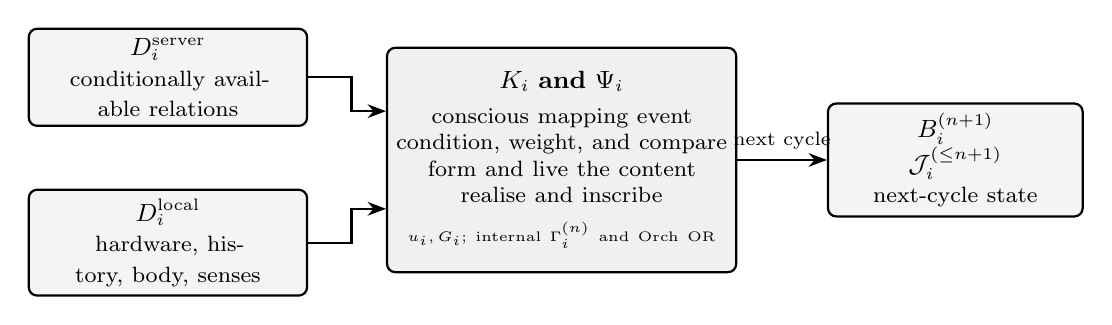
\begin{tikzpicture}[
  >=Stealth, thick,
  inbox/.style={draw, rounded corners=3pt, fill=gray!9,
                text width=3.3cm, minimum height=1.2cm,
                align=center, font=\small},
  procbox/.style={draw, rounded corners=3pt, fill=black!6,
                  text width=4.2cm, minimum height=2.85cm,
                  align=center, font=\small},
  outbox/.style={draw, rounded corners=3pt, fill=gray!9,
                 text width=3.0cm, minimum height=1.3cm,
                 align=center, font=\small}
]
\node[inbox] (server) at (0, 1.05)
  {$D_i^{\mathrm{server}}$\\\footnotesize conditionally available relations};
\node[inbox] (local) at (0,-1.05)
  {$D_i^{\mathrm{local}}$\\\footnotesize hardware, history, body, senses};
\node[procbox] (ki) at (5.0, 0)
  {{\bfseries $K_i$ and $\Psi_i$}\\[3pt]\footnotesize conscious mapping event\\
   \footnotesize condition, weight, and compare\\
   \footnotesize form and live the content\\
   \footnotesize realise and inscribe\\[3pt]
   \tiny $u_i,G_i$; internal $\Gamma_i^{(n)}$ and Orch~OR};
\node[outbox] (out) at (10.0, 0)
  {$B_i^{(n+1)}$\\$\mathcal J_i^{(\leq n+1)}$\\\footnotesize next-cycle state};
\draw[->] (server.east) -- ++(0.55,0) |- ([yshift=0.62cm]ki.west);
\draw[->] (local.east) -- ++(0.55,0) |- ([yshift=-0.62cm]ki.west);
\draw[->] (ki.east) -- node[above,font=\scriptsize] {next cycle} (out.west);
\end{tikzpicture}
\caption{The complete Interpreter Model. Local data and conditionally available
server data meet in one conscious mapping event. $\Psi_i$ is the content formed and
lived in that event, not an output viewed by a later observer. Inscription supplies
the changed conditions of the next cycle.}
\label{fig:model_map}
\end{figure}

\subsection{From a conscious event to a continuing self}
\label{sec:self}

What does this mean for the one who experiences? In this model, making the image is
already experiencing it. The one mapping that
forms $\Psi_i$ is the event in which the image is lived, so that perspective arises
in the forming itself and not in any later viewing. No inner viewer is needed to whom
the image is shown. The model does not forbid a homunculus; it simply has no work
left for one. Because this perspective is made
new in each event and is not held by a standing observer, the continuity we call the
self is the ordered sequence of these events, each of which inherits the
configuration left by the one before.

Within this account, the ego belongs to $B_i$. It is the learned biographical form
that shapes ownership, expectation, and the next rendering, whereas $K_i$ is the
active process. Temporary unconsciousness can interrupt the current rendering while
the local structure, from which continuity is rebuilt, stays in place. Structural
degeneration reaches further, because it changes the self-model that is available.

Two people can share a relation, a song they both know or a day they spent together,
and still each keeps their own perspective on it, because perspective stays with the
locally ordered sequence of mappings. How one shared relation becomes two individual
mappings is given in Eq.~\eqref{eq:shared_relation_local_mappings}; pattern dominance
and coherence are defined in
Eqs.~\eqref{eq:relational_dominance}--\eqref{eq:weighted_convergence}.

Can this be measured? For memory, it can. When the number of relations is held equal,
a single cue brings back the rest of an event more reliably if every element of the
event is linked to every other than if the elements form an open chain
\citep{horner2015}. Studies with naturalistic stories go one step further. How
central an event is to the meaning and to the chain of cause and effect, measured
independently, predicts how well it is recalled later, how strongly the hippocampus
takes part, and how similar the brain patterns for that event become across
different listeners \citep{leechen2022}. These measurements fix the direction of the
weighting rule independently of the model calculation. The measured coefficients and
their transformations are given in Table~\ref{tab:relational_convergence_data}.

In the next chapter we put the model under stress. Ordinary perception serves as the
baseline, and each test changes one measurable part of the process and asks whether the
same equation still organises the observations.

\emph{Continued interpretation gives experience a history and a perspective,
bringing us back to the thinking self with which Descartes began.}

\section{Clinical Perturbations and Dissociations}
\label{sec:applications}

A model of consciousness is only as good as what it can tell us about real people. In
this chapter we therefore take it into the clinic and the laboratory. We look at when
an image forms, what anaesthesia and heat do to it, and what happens when single steps
of the cycle fail.

\subsection{Timing of conscious rendering}

When we smell coffee, when exactly do we know that it is coffee? The nose has
registered something well before we can name it. Local production accounts can follow
the processing that comes before awareness, but they still have to explain how the
experienced present is put together from it. \emph{Mind Time} gives us an empirical
point of comparison: conscious placement follows earlier neural processing and
develops over a measurable interval \citep{libet2004}.

Smell is a good place to look, because here the two moments can be told apart: early registration and
conscious identification show up in separate responses \citep{arpaia2022}, and
recurrent piriform circuits help to stabilise the representation as it emerges
\citep{bolding2020}. Three studies give timing values, which we take from their
published abstracts. Harada et al. (50 stimuli, OERP) measured peaks near 350 and
700 ms, giving an interpeak interval of 350 ms \citep{harada2003}. Kayser et al. (32
patients, 35 controls, unirhinal H$_2$S) found an N1 sink at 305 ms and a P2 source
at 630 ms, which are 325 ms apart \citep{kayser2010}. Walla et al. (20 participants,
MEG) reported an early effect at 200--500 ms with and without perceived odour. When
their data were divided by reported odour awareness, a later effect at 600--900 ms
was stronger in the group with conscious perception, and the centres of the two
windows lie 400 ms apart \citep{walla2002}. Across the three studies, the comparison
range is 325--400 ms.

How does the model arrive at a time of this order? It works on two levels, and each
is calculated on its own.

\paragraph{The nerve cell.}
A neuron that has just fired is slower to fire again, because its recent history holds
it back for a moment. The adaptive Hodgkin--Huxley/AdEx model captures this with one
adaptive current, $w_i(t)$. With the published regular-spiking parameters, its
stationary equations give the rheobase, the smallest input that makes the cell fire,
and a sweep over the whole input range $I/I_{\mathrm{rheo}}$ shows how one
spike-triggered increment of $w_i(t)$ delays the next local trigger
\citep{brettegerstner2005}. The parameters and numerical controls are given in
Table~\ref{tab:adaptive_trigger_provenance}, and the resulting latency sweep appears
in Figure~\ref{fig:adaptive_trigger_sensitivity}.

\paragraph{The carrier.}
Inside the cell, the Orch~OR calculation follows the microtubule from the driven
recruitment of Eq.~\eqref{eq:coupled_frohlich_recruitment} up to the threshold at
which the reduction happens. The adaptation of the neuron stays on the AdEx level. On
the carrier side, the finite width of the atomic nuclei sets a plateau that limits how
the reduction scales. The stationary carrier counts and saturation limits are given in
Table~\ref{tab:geometric_eg_profiles}; the comparison values from the historical
Hameroff--Penrose calculation are kept separately in
Table~\ref{tab:historical_hp_anchors}.

\paragraph{A combined test.}
An experiment that records early registration, conscious report, neural state, and
odour familiarity in the same participants would test the measured range, the
adaptive response, and the carrier scaling together.

\subsection{Anaesthesia and reduced sensory anchoring}

Why do people under ketamine often report vivid, dreamlike experience, while propofol
usually leaves nothing to report? Both are anaesthetics, yet they leave very different
states behind. In the model they act at different points. In dissociative
anaesthesia, the current input from the senses and the body, $I_{\mathrm{syn}}$, loses
its usual dominance while the mapping $K_i$ keeps running. The result is vivid
experience, coloured by the person's biography, with only a weak anchor in the body.
Suppressive anaesthesia reaches the process at another point: stable coupling stops,
and no experiential image is fixed. Ketamine and propofol thus mark the two limits of
the model, with REM sleep and deep coma as their neighbours.

Microtubules connect this distinction with interventions that can be measured.
Modelling relates anaesthetic potency to collective tubulin oscillations
\citep{craddock2017}, and measurements show that electronic energy migrates in
microtubules and that isoflurane and etomidate damp it \citep{kalra2023}.
Interventions that modulate microtubules alter isoflurane sensitivity, induction, or
emergence in mice \citep{li2025}, and in experiments with rats and mice,
stabilisation with epothilone~B delayed the loss of responsiveness under anaesthesia
\citep{khan2024,huang2026}. The study designs, doses, delays, significance values,
and effect sizes are given in Table~\ref{tab:biological_carrier_constraints}. Within
the model, a change in the carrier changes the transition at which stable rendering
is lost. The separate mass-density inputs are given in
Table~\ref{tab:orch_or_parameter_provenance}.

\subsection{Thermal load as a stage-resolved test}

Temperature lets us disturb the operating state of the system without first taking
away its sensory input. During a heat wave, a field study followed 44 students, of
whom twenty lived without air conditioning at a mean indoor temperature of
26.3\,${}^{\circ}$C and 24 lived with air conditioning at 21.4\,${}^{\circ}$C. The
difference between their changes from baseline was 13.4 percent for Stroop reaction
time and 13.3 percent for two-digit arithmetic reaction time. The group without air
conditioning also showed a 9.9 percent relative reduction in Stroop throughput, and
its fitted indoor-temperature curve had an optimum near 22\,${}^{\circ}$C
\citep{cedenolaurent2018}. This was a real indoor exposure in which heat and humidity
acted together, whereas controlled hyperthermia lets us follow the same disturbance
from brain temperature to electrical activity and behaviour.

During passive heating, brain temperature rose while grey-matter perfusion, cortical
motor activity, and Stroop accuracy fell \citep{tan2024heat}. The EEG studies show
where in the processing sequence the change happens. The early N100 response stayed
stable, while the later P300 response came earlier and with less amplitude, and
sufficient whole-body cooling moved the visual response back towards baseline
\citep{shibasaki2016heat,nakata2021heat}. The measured temperatures, latencies,
amplitudes, behavioural changes, and confidence intervals are given in
Table~\ref{tab:thermal_processing_chain}.

\begin{table}[t]
\centering
\footnotesize
\renewcommand{\arraystretch}{0.97}
\begin{tabular}{@{}
>{\raggedright\arraybackslash}p{2.8cm}
>{\raggedright\arraybackslash}p{3.35cm}
>{\raggedright\arraybackslash}p{3.9cm}
>{\raggedright\arraybackslash}p{3.2cm}@{}}
\toprule
Stage and measurement & Comparison under heat & Relative P300 change [95\% CI] & Place in the processing chain \\
\midrule
Thermal state: $^{1}$H-MRS and MRI
& brain temperature $+0.9\pm0.5\,{}^{\circ}$C; grey-matter perfusion lower ($p=0.016$); cortical motor BOLD lower
& --
& the controlled disturbance reaches the brain \citep{tan2024heat} \\[2pt]
Early registration: auditory N100
& latency and amplitude unchanged at about $+2.0\,{}^{\circ}$C oesophageal temperature
& control\textsuperscript{b}
& initial auditory arrival remains available \citep{shibasaki2016heat} \\[2pt]
P300 latency: auditory and visual
& auditory time control $287\rightarrow$ heat stress $278$ ms at the third session; visual $380.53\rightarrow346.19$ ms and $383.78\rightarrow355.81$ ms
& auditory $-3.14\%$\textsuperscript{b}; visual congruent $-9.03\%$ [$-13.08,-4.71$] and incongruent $-7.29\%$ [$-10.41,-4.34$]\textsuperscript{a}
& later classification or evaluation occurs earlier \citep{shibasaki2016heat,nakata2021heat} \\[2pt]
P300 amplitude: auditory and visual
& auditory $12.2\rightarrow8.3\,\mu$V; visual $13.17\rightarrow11.09\,\mu$V and $12.14\rightarrow9.59\,\mu$V
& auditory $-31.97\%$\textsuperscript{b}; visual congruent $-15.78\%$ [$-24.05,-5.80$] and incongruent $-20.98\%$ [$-31.30,-10.50$]\textsuperscript{a}
& the later task-related electrical response is smaller \citep{shibasaki2016heat,nakata2021heat} \\[2pt]
Behavioural output: reaction time and accuracy
& visual reaction time $-8.9$ and $-9.2$ percent; overall Stroop accuracy lower after passive heating ($p=0.017$)
& --
& faster output can accompany lower response integrity \citep{nakata2021heat,tan2024heat} \\
\bottomrule
\end{tabular}
\caption{A cross-study sequence from thermal brain state to behavioural output. The
EEG comparisons use auditory and visual tasks, while MRI describes the wider
operating state of the brain.}
\label{tab:thermal_processing_chain}
\vspace{2pt}
\parbox{\textwidth}{\scriptsize \textsuperscript{a}All Nakata visual ERP values are
from Pz; the intervals are paired 95 percent bootstrap intervals calculated from
participant data. \textsuperscript{b}Shibasaki reported means with standard errors,
so no relative-change confidence intervals were calculated; the unchanged N100
remains as the control.}
\end{table}

Heat therefore does not make the brain slower across the board. Local evaluation
finishes earlier, but the electrical response that goes with it becomes smaller. Warmer cortical neurons explain part of this in an ordinary biological way,
because sodium-channel inactivation speeds up, action potentials shorten, and the
firing rate can rise for the same input \citep{yu2012warm}. In the model, thermal
load therefore changes both the current biological state in $B_i(t)$ and the set of
branches that the hardware can realise. A quicker answer can be formed from a weaker
mapping, which is why response speed and response integrity move in opposite
directions in Table~\ref{tab:thermal_processing_chain}.

The carrier level offers a second and independent test.
The shear modulus of microtubules depends on temperature \citep{kis2008}, and
Equations~\eqref{eq:coupled_frohlich_recruitment}
and~\eqref{eq:adaptive_or_trigger} convert a measured change in the carrier into a
change of recruitment and of the reduction interval. The EEG values describe the
local evaluation around that event. An experiment that records brain temperature,
carrier state, P300, and accuracy together would separate the two timescales and
show how much each one contributes.

\subsection{Neurological dissociations of the mapping process}

So far we have reached the cycle with a drug and with heat. Epothilone~B acts at one
point of the cycle, and heat changes the operating state of the whole sequence. What
about the other steps? This is where the model places the neurological dissociations,
and it ties a change at each step to a different clinical pattern.

The medical value of the model begins where conditions that look alike from outside
come from different disturbances inside the mapping cycle. A patient may fail to form
a stable image, to connect it with stored identity, to keep it as memory, or to
express an experience that is still present, and a missing outward response does not
tell us which of these operations has failed. Once the disturbances are placed at
different points of the same process, the clinical question changes from whether
consciousness is present to where the mapping has been disturbed and which functions
are still available. The clinical dissociations and their measured patterns are
given in Table~\ref{tab:state_classification}.

\begin{table}[H]
\centering
\footnotesize
\renewcommand{\arraystretch}{0.97}
\begin{tabular}{@{}
>{\raggedright\arraybackslash}p{2.4cm}
>{\raggedright\arraybackslash}p{2.75cm}
>{\raggedright\arraybackslash}p{3.85cm}
>{\raggedright\arraybackslash}p{3.8cm}@{}}
\toprule
Model operation & Clinical dissociation & Consequence in the mapping & Measured clinical pattern \\
\midrule
Temporal integration
& akinetopsia and palinopsia
& successive visual states fail to join as movement, or an earlier state enters the next mapping again
& motion fragments while other modalities remain available, or an image persists after its stimulus ends \citep{zihl1983,stafuzza2018} \\[2pt]
Current recruitment
& absence seizure
& the current mapping is interrupted or loses selected operations
& response initiation can fail while short-term storage remains available \citep{vuilleumier2000} \\[2pt]
Form-to-identity assignment
& associative agnosia or prosopagnosia
& visible form and identity fail to converge in the mapping
& elementary vision may remain while object or face recognition fails \citep{delvenne2004} \\[2pt]
Familiarity weighting
& Capgras syndrome
& recognised identity and felt familiarity are assigned incompatible sources,
separating familiarity from identity recognition
& a familiar face is recognised without the usual autonomic distinction \citep{ellis1997} \\[2pt]
Durable write
& anterograde amnesia
& an image is experienced but is not consolidated into later local history
& present function remains while new lasting episodic storage is severely impaired \citep{scoville1957} \\[2pt]
Behavioural expression
& UWS, MCS, and akinetic mutism
& a realised mapping remains available without initiating an ordinary bedside response
& covert command following or auditory cognitive responses can remain when spontaneous action is absent \citep{monti2010,naccache2004} \\
\bottomrule
\end{tabular}
\caption{Six classes of clinical dissociation placed at different operations of one
personalised mapping cycle.}
\label{tab:state_classification}
\end{table}

\subsection{Operational disruption, data gaps, and resynchronisation}
\label{sec:reconstruction}

Anaesthetic agents and sensory loss allow us to disturb single operations of the
mapping cycle under controlled conditions, and the pattern that results is more
useful than one scale running from awake to unconscious. A patient may process an
event without forming a later memory. Perceptual content may appear when current
sensory input is missing, and experience may remain while body, place, and the
connection to the surroundings become unstable. During recovery, these functions do
not have to return at the same time.

The model has names for these familiar clinical separations. WRITE is the formation
of durable memory, INTERPRET/FILL is the completion of perceptual content, and
ANCHORING assigns that content to a body and an environment. REBOOT/SYNC is the
staged recovery of an integrated mapping, and the operation profile records how far
agent and dose reach each of these functions.

A sync begins when bodily and sensory processing returns but the recovered present
no longer joins cleanly to the last stable local state. The interval between the two
is the data gap $G_i$. The interpreter compares what the body can supply again, what
its local history already contains, and the conditionally available relations from
the server, and it then maps this material back onto the person's senses, bodily
position, and local order of time.

The mapping is the whole lived situation and much more than a visual
picture, because it includes sensory form, bodily position, spatial and temporal
order, affect, meaning, source, and perspective. A gap does not require every local
process to stop. If the returning anchors stay weak or contradict each other, the
sync can still form a coherent experience while placing its source, viewpoint, or
time incorrectly. The gap is defined in Eq.~\eqref{eq:mapping_gap}; its repair and
any remainder carried into the next cycle are given in
Eqs.~\eqref{eq:resynchronisation_map} and~\eqref{eq:residual_mapping_gap}. The
experimental and clinical interventions that separate these operations are given in
Table~\ref{tab:operational_disruption}.

\begin{table}[H]
\centering
\footnotesize
\renewcommand{\arraystretch}{0.98}
\begin{tabular}{@{}
>{\raggedright\arraybackslash}p{2.58cm}
>{\raggedright\arraybackslash}p{3.15cm}
>{\raggedright\arraybackslash}p{4.2cm}
>{\raggedright\arraybackslash}p{2.87cm}@{}}
\toprule
Operation & Experimental or clinical intervention & Observation & Model relation \\
\midrule
\textbf{WRITE} into $B_i$
& midazolam; isolated-forearm testing during anaesthesia
& sedation can lift while amnesia remains; 12 of 260 patients responded during intended anaesthesia and none later reported explicit recall
& current processing without a durable local write \citep{curran1991,sanders2017} \\[2pt]
\textbf{INTERPRET / FILL} in $K_i$
& severe sight loss; Charles Bonnet syndrome
& formed visual content follows specialised visual regions; activity can build in early visual cortex before the reported image
& the visual part of an experiential image forms despite missing current visual input \citep{ffytche1998,hahamy2021} \\[2pt]
\textbf{ANCHORING} through $B_i(t)$ and $I_{\mathrm{syn}}(t)$
& ketamine in rubber-hand and disconnected-consciousness paradigms
& vivid experience remains while body ownership, hand location, and connection to the environment become unstable
& interpretation continues with weakened bodily and environmental weights \citep{morgan2011,sarasso2015} \\[2pt]
\textbf{REBOOT / SYNC} of $K_i$ across $G_i$
& emergence after three hours of isoflurane anaesthesia
& frontoparietal dynamics return before responsiveness; cognitive functions then recover in a measured sequence
& stable local mapping is rebuilt through an ordered recovery \citep{mashour2021} \\[2pt]
\textbf{OPERATION PROFILE}
& agent $\times$ dose
& writing, filling, anchoring, and recovery do not fail together or to the same degree
& the disturbance profile follows the operation reached and the depth of the intervention \\
\bottomrule
\end{tabular}
\caption{Experimental and clinical anchors for operations that can separate during a disturbance
of the mapping cycle.}
\label{tab:operational_disruption}
\end{table}

\section{Discussion and Conclusion}
\label{sec:discussion}

At the start of this paper we asked why a shared world is experienced so differently
by each of us. The model finds the answer where two sides meet. The shared field carries relations
without a viewpoint, and the living system contributes the history through which a
viewpoint can form. Their meeting in $K_i$ creates the available branches, physical
fixation makes one event real, and inscription carries it into the next cycle. In
this way a relation enters a living history and becomes a situated image.

Each application changes this operation at a different point. Timing asks when an
image forms, anaesthesia reaches either the sensory weighting or the carrier, and
thermal load separates early registration from the strength of later processing.
The neurological dissociations and the controlled interruptions then show that
writing, filling, anchoring, and recovery can fail one at a time. For medicine this
may be the most useful consequence of the model. When a patient does not respond, the
more useful question becomes where in the cycle the mapping has been disturbed and
which of its operations are still working.

On the physical side, the model does not borrow its numbers. The gravitational
self-energy that sets the reduction interval was calculated directly from the atomic
coordinates of the tubulin dimer \citep{lowe2001}, without calibrating it to any
collapse time. It grows almost linearly with the number of recruited dimers, so no
hidden $N^2$ amplification is required, and for event intervals between 25 and
500~ms it places the carrier population between about $10^9$ and $10^{12}$ dimers,
depending on how the nuclear profile is read (Table~\ref{tab:geometric_eg_profiles}).

These results lead to tests that can be carried out with existing methods. When two
carrier states are characterised independently, the ratio of their event intervals
should follow the inverse ratio of their gravitational self-energies, as stated in
Eq.~\eqref{eq:or_ratio_test}. Stabilising microtubules with epothilone~B already
delays the loss of responsiveness under anaesthesia \citep{khan2024,huang2026}, and
the model predicts that the size of this delay follows the measured change in the
carrier. Under heat, the speed and the integrity of a response should keep moving in
opposite directions for as long as early registration stays intact. Relational
structure that is measured before recall should predict how strongly and how quickly
a memory converges, following the preregistered protocol in
Table~\ref{tab:relational_convergence_protocol}. In each of these tests the entering
state is measured first, and its consequence is derived before it is compared with
what the person reports.

Some questions remain open, and they are worth naming. The weighting function
$\mathcal W_i$ is fixed in the direction of its dependencies but not yet in its exact
form, and the recruitment of carrier domains is treated as a simple onset once the
gain becomes positive. The relational field is not observed directly. It is inferred
from what its relations make possible, which means that the tests above, and not a
look at the server, will decide whether the model holds.

We began with a shared world and the many ways in which it is experienced, and the
model returns to this observation through one operation. Relations supply what can be
mapped, while a living history gives them a world and a perspective. In their
meeting, world and observer appear together. The observer is part of what the meeting
forms, so no homunculus is needed to watch it.


\appendix
\section{Notation and Definitions}
\label{app:notation}

\begin{table}[H]
\centering
\scriptsize
\renewcommand{\arraystretch}{0.90}
\begin{tabular}{p{3.0cm}p{9.8cm}}
\toprule
Symbol & Meaning in the Interpreter Model \\
\midrule
$\varphi_Q$ & Timeless relational field, represented in the formal model by the relational sector of the global quantum state and used as the shared server basis. \\
$B_i$ & Locally stored life history and the resulting individual configuration of interpreter $i$. \\
$B_i(t)$ & Current bodily, adaptive, and attentional configuration of the local interpreter. \\
$I_{\mathrm{syn}}(t)$ & Current locally available sensory and bodily input. \\
$D_i^{\mathrm{local}}$ & Complete local side: $B_i$, $B_i(t)$, $I_{\mathrm{syn}}(t)$, and the physical client configuration. \\
$\Gamma_{\mathrm{server}}$ & Timeless network extracted from the correlation effects of the global relational state. \\
$\Gamma_i^{(n)}$ & Weighted projection of $\Gamma_{\mathrm{server}}$ produced by interpreter $i$ during mapping cycle $n$. \\
$\mathcal J_i^{(\leq n)}$ & Realised relations encountered up to event $n$ in the local causal order of interpreter $i$. \\
$\hat C_\gamma$ & Positive effect representing relation $\gamma$ in the relational sector, with $0\leq\hat C_\gamma\leq I$. \\
$\Pi_i^{(n)}$ & Local conditioning projector fixed by interpreter $i$'s causal address and event index. \\
$\omega_{i\gamma}^{(n)}$ & Effective weight of server relation $\gamma$ in interpreter $i$'s current mapping cycle. \\
$e_{i\gamma}^{(n)},m_{i\gamma}^{(n)}$ & Conditionally available relation strength and its local mappability factor. \\
$a_{i\gamma}^{\mathrm{bio}},\mu_{i\gamma}$ & Biographical affinity and pattern overlap used in local weighting. \\
$\operatorname{dist}_{h_i}(p_i,p_\gamma),|\Delta s_{i\gamma}|$ & Invariant distance on the local rest slice and local proper-time separation from relation $\gamma$. \\
$H_i$ & Biological hardware presently available to interpreter $i$. \\
$D_i^{\mathrm{server},(n)}$ & Conditionally available server-side relation data $(\gamma,e_{i\gamma}^{(n)})$ passed to mapping cycle $n$ before local mappability and weighting are applied. \\
$\mathfrak B_i^{(n)}$ & Relation-indexed carrier branches that are both available in cycle $n$ and physically realisable by the current biological hardware. \\
$u_i^\mu$ & Future-directed local timelike vector $dx_i^\mu/ds_i$ that orders mapped relations along interpreter $i$'s physical worldline; $s_i$ is local proper time. \\
$h_{\mu\nu}^{(i)}$ & Induced spatial metric on the local rest slice $\Sigma_i$ orthogonal to $u_i^\mu$. \\
$K_i$ & One bidirectional conditioning, comparison, spacetime mapping, physical realisation, rendering, and inscription process. \\
$E_G,e_G$ & Total Penrose gravitational self-energy difference of two Orch-OR branch mass profiles, and the corresponding single-dimer contribution used in the geometric scaling calculation. \\
$\sigma_\nu,\Delta R$ & Width of nuclear Gaussian profile $\nu$ and displacement between its two branch positions. \\
$\tau_i$ & Locally measured collapse interval of one rendering event. \\
$w_i(t)$ & Adaptive neuronal current that carries recent firing history and changes the effective local trigger. \\
$q_{ik}(s)$ & Occupation of the lowest collective vibrational mode in candidate carrier domain $k$. \\
$n_{ik},\Omega_i(s),N_i(s)$ & Dimer population of domain $k$, set of recruited domains, and total recruited dimer count $\sum_{k\in\Omega_i(s)}n_{ik}$ at local time $s$. \\
$A_i(s)$ & Accumulated dimensionless Orch-OR action $\hbar^{-1}\int_0^sE_G(s')ds'$. \\
$N_i^*$ & Total recruited dimer count immediately before the endogenous Orch-OR threshold is reached. \\
$N_G^*(\tau_i)$ & Stationary carrier count obtained from the independently evaluated geometric $E_G$. \\
$N_{\mathrm{HP}}^*(\tau_i)$ & Literature-anchored carrier count for interval $\tau_i$ in the additive Hameroff--Penrose benchmark. \\
$\Psi_i$ & Experiential image formed during $K_i$; the mapping event itself is conscious. \\
$G_i$ & Data gap detected in the local state after a mapping disruption. \\
$C_i$ & Maximum weighted convergence of a relational pattern in the current mapping cycle. \\
$\mathcal F_i$ & Fidelity of source, perspective, event detail, and temporal assignment; $\mathcal F_{i,\mathrm{event}}$ denotes event-detail fidelity. \\
$T_{i,\mathrm{resp}}$ & Measured interval from cue onset to a stable response in the prospective relational-convergence test. \\
\bottomrule
\end{tabular}
\caption{Notation used throughout the paper.}
\label{tab:notation}
\end{table}

\section{Neurodynamic and Biological Implementation}
\label{app:neurodynamic}

\subsection{Carrier constraints and source values}

\begin{table}[H]
\centering
\footnotesize
\begin{tabular}{@{}
  >{\raggedright\arraybackslash}p{3.0cm}
  >{\raggedright\arraybackslash}p{5.2cm}
  >{\raggedright\arraybackslash}p{5.0cm}@{}}
\toprule
Source & System or intervention & Result used here \\
\midrule
\citet{frohlich1968} & metabolically driven polar structures & collective vibrational modes \\
\citet{zhang2019frohlich,wang2022frohlich} & driven molecular vibrations & pump threshold, gain--loss dynamics, and nonequilibrium phase transition \\
\citet{preto2026} & driven classical protein-mode Hamiltonian in a 300 K bath & Fr\"ohlich-type condensation across common coupling rescaling from $0.01$ to $1$; bath-mediated low-frequency nonlinear coupling required \\
\citet{engel2007} & photosynthetic complex (FMO) at 77 K & long-lived electronic coherence in energy transfer \\
\citet{panitchayangkoon2010,collini2010} & photosynthetic complexes at physiological and ambient temperature & warm biological coherence \\
\citet{ishiwata2026} & pentacene molecular spins in nanocrystals inside living cells & intracellular Rabi control and spin echo; $T_2\sim1\,\mu\mathrm{s}$ and $T_1\sim75\,\mu\mathrm{s}$ \\
\citet{babcock2024} & tryptophan networks and tubulin assemblies & ultraviolet superradiant modes and enhanced quantum yield \\
\citet{mavromatos2025} & ordered-water/microtubule QED cavity & estimated decoherence interval $10^{-7}$--$10^{-6}$ s \\
\citet{craddock2017} & collective tubulin-mode model & anaesthetic-dependent mode change \\
\citet{kalra2023} & purified microtubules; isoflurane and etomidate & $D=(3.15\pm0.10)\times10^{-5}\,\mathrm{cm^2\,s^{-1}}$; $L=6.64\pm0.10$ nm; reduced transport \\
\citet{khan2024} & epothilone~B arm, eight male rats (12 animals in the study); 0.75 mg/kg; 4 percent isoflurane & loss of righting reflex delayed 69 s; permutation $t$-test $p=0.0016$; $d=1.9$ \\
\citet{li2025} & prolonged microtubule-modulating drug treatment in mice & drug-specific shifts in isoflurane sensitivity, induction, and emergence \\
\citet{huang2026} & mice; one 8 mg/kg epothilone~B dose & following-day delay 29 s; $d=0.8$ \\
\bottomrule
\end{tabular}
\caption{Theoretical, experimental, and intervention results used in the biological
carrier account.}
\label{tab:biological_carrier_constraints}
\end{table}

\subsection{Macroscopic neural field}

The neural population follows a one-population Wilson--Cowan reduction
\citep{wilsoncowan1972}.
\begin{equation}
  \tau_E \frac{\partial E(\mathbf{x},t)}{\partial t}
  = -E(\mathbf{x},t)
  + \mathcal S\left[
      \int W_E(\mathbf{x}-\mathbf{x}')E(\mathbf{x}',t)\,d^3x'
      + P(\mathbf{x},t)
    \right].
  \label{eq:wilsoncowan}
\end{equation}
\noindent Here $E$ is the population activity, $\tau_E$ the population time
constant, $W_E$ the spatial kernel, and $\mathcal S$ a dimensionally normalised
sigmoid. $P$ is the local sensory, bodily, and realised-carrier drive.

\subsection{Adaptive single neuron}

The single neuron follows the Adaptive Exponential Integrate-and-Fire reduction
\citep{hodgkinhuxley1952,brettegerstner2005}.
\begin{align}
  C_m \frac{dV}{dt} &=
    -g_L(V-E_L)
    + g_L\Delta_T\exp\left(\frac{V-V_T}{\Delta_T}\right)
    - w_i + I_{\mathrm{ext}},
  \label{eq:adex_V}\\
  \tau_w \frac{dw_i}{dt} &= a(V-E_L)-w_i.
  \label{eq:adex_w}
\end{align}
\noindent At each spike the neuron is reset by $V\leftarrow V_r$ and
$w_i\leftarrow w_i+b$. With $w_i$ held fixed, the exponential term places the
subthreshold saddle at $V=V_T$. This gives the effective trigger current
\begin{equation}
  I_{\theta,i}^{\mathrm{eff}}(t)
  \simeq g_L(V_T-E_L-\Delta_T)+w_i(t).
  \label{eq:adaptive_trigger}
\end{equation}
\noindent The time $t$ is identified with the proper time $s_i$ on the local
worldline.

\section[Quantum-Gravitational Coupling and Derivations]
{Quantum-Gravitational Coupling\\and Derivations}
\label{app:quantum_coupling}

\subsection{Timeless state and server relations}

The starting point is the Wheeler--DeWitt constraint \citep{dewitt1967}.
\begin{equation}
  \hat H|\Phi\rangle=0,
  \qquad
  \hat H=\hat H_{\mathrm{grav}}+\hat H_{\mathrm{matter}}.
  \label{eq:wdw}
\end{equation}
Let $\rho_Q$ be the normalised state induced by $|\Phi\rangle$ on the relational
sector $\varphi_Q$. The server notation is the correlation map
\begin{equation}
  e_\gamma=\operatorname{Tr}(\rho_Q\hat C_\gamma),
  \qquad
  \Gamma_{\mathrm{server}}
  =\left\{\gamma:e_\gamma>0\right\},
  \qquad 0\leq\hat C_\gamma\leq I.
  \label{eq:server_relation_encoding}
\end{equation}
At the local address selected by $\Pi_i^{(n_i)}$, the relation strength passed to
$K_i$ is
\begin{equation}
  e_{i\gamma}^{(n_i)}=
  \frac{\operatorname{Tr}\!\left(
    \Pi_i^{(n_i)}\hat C_\gamma\Pi_i^{(n_i)}\rho_Q
  \right)}
  {\operatorname{Tr}\!\left(\Pi_i^{(n_i)}\rho_Q\right)},
  \qquad \operatorname{Tr}\!\left(\Pi_i^{(n_i)}\rho_Q\right)>0.
  \label{eq:server_relation_read}
\end{equation}
The complete server-side input to cycle $n_i$ is therefore
\begin{equation}
  D_i^{\mathrm{server},(n_i)}=
  \left\{(\gamma,e_{i\gamma}^{(n_i)}):
  \gamma\in\Gamma_{\mathrm{server}},\ e_{i\gamma}^{(n_i)}>0\right\}.
  \label{eq:available_server_data}
\end{equation}
It contains conditionally available relations and their read strengths. Local
mappability, effective weights, and the projection $\Gamma_i^{(n_i)}$ are formed
only after these data enter $K_i$.
The realised event changes the local configuration and local event history:
\begin{equation}
  B_i^{(n_i+1)}=B_i^{(n_i)}\oplus\Psi_i^{(n_i)},
  \qquad
  \mathcal J_i^{(\leq n_i+1)}
  =\mathcal J_i^{(\leq n_i)}\cup\{\gamma_i^{(n_i)}\},
  \qquad \gamma_i^{(n_i)}\in\Gamma_{\mathrm{server}}.
  \label{eq:server_relation_write}
\end{equation}
\noindent Here $\oplus$ denotes local incorporation, $\gamma_i^{(n_i)}$ the realised
relation, and $n_i$ the local causal event index. The global $\rho_Q$ and
$\Gamma_{\mathrm{server}}$ carry no $n_i$ evolution. Equation~\eqref{eq:server_relation_write}
is the internal read/write description of a relation in the ordered local history,
not evolution under an external server clock \citep{pagewootters1983}.

\subsection{CDT and the local time vector}

CDT sums over causal triangulations \citep{ambjorn2004}.
\begin{equation}
  Z_{\mathrm{CDT}}=
  \sum_{T\in\mathcal T_{\mathrm{causal}}}\frac{1}{C_T}
  \exp\!\left[-\frac{S_E[T]}{\hbar}\right].
  \label{eq:cdt}
\end{equation}
\noindent Here $C_T$ is the symmetry factor and $S_E[T]$ the Euclideanised
discretised action. Each $T\in\mathcal T_{\mathrm{causal}}$ is an admissible
foliation and gluing.

Only an effective continuum geometry is passed forward from the CDT ensemble.
\begin{equation}
  \left\{T\in\mathcal T_{\mathrm{causal}}\right\}_{Z_{\mathrm{CDT}}}
  \xrightarrow{\ \mathcal C_\ell\ }
  (\overline M,\overline g_{\mu\nu}^{(\ell)}),
  \qquad \ell\gg a_{\mathrm{CDT}}.
  \label{eq:cdt_coarse_geometry}
\end{equation}
\noindent Here $\mathcal C_\ell$ is the coarse-graining in a semiclassical CDT
sector, and $a_{\mathrm{CDT}}$ is the lattice scale
\citep{ambjorn2004,benedetti2007}.

On the resulting patch, the local tetrad and spin frame are normalised by
\begin{equation}
  \overline g_{\mu\nu}^{(\ell)}=
  e_{\mu}^{AA'}(\ell)e_{\nu}^{BB'}(\ell)\epsilon_{AB}\epsilon_{A'B'},
  \qquad
  \xi_{i,\ell}^{AA'}=e_{\mu}^{AA'}(\ell)\xi_i^\mu.
  \label{eq:cdt_spinframe}
\end{equation}
\noindent Here $\overline g_{\mu\nu}^{(\ell)}$ is the effective local Lorentzian
metric and $e_\mu^{AA'}$ the spin frame. $\xi_{i,\ell}^{AA'}$ is the bispinor form
of the Riemann-normal coordinate $\xi_i^\mu\in T_{p_i}\overline M$
\citep{speziale2012}.

The future-directed local tangent of the client's worldline is
\begin{equation}
  u_i^\mu=\frac{dx_i^\mu}{ds_i},
  \qquad
  \overline g_{\mu\nu}^{(\ell)}u_i^\mu u_i^\nu=-1
  \quad(c=1),
  \label{eq:local_time_vector}
\end{equation}
\noindent Here $s_i$ is the proper time and $\tau_i$ the local collapse interval. A
shared relation is weighted on each of the two worldlines,
$\gamma_{ij}\mapsto(\omega_{i\gamma_{ij}},\omega_{j\gamma_{ij}})$.

Within the normal neighbourhood of the local event, the same geometry defines the
spatial rest section used by the branch-density calculation:
\begin{equation}
  h_{\mu\nu}^{(i)}=
  \overline g_{\mu\nu}^{(\ell)}+u_{i\mu}u_{i\nu},
  \qquad
  h_{\mu\nu}^{(i)}u_i^\nu=0,
  \qquad
  d\mu_{h_i}=\sqrt{\det h_{mn}^{(i)}}\,d^3x .
  \label{eq:cdt_rest_slice}
\end{equation}
\noindent Here $h_{mn}^{(i)}$ is the positive spatial metric induced on the local
section $\Sigma_i$ orthogonal to $u_i$. Its Green kernel is fixed by
\begin{equation}
  -\Delta_{h_i}\mathcal G_{h_i}(x,y)=4\pi\delta_{h_i}(x,y),
  \qquad
  \mathcal G_{h_i}(x,y)
  \xrightarrow{\ \ell^2\|\operatorname{Riem}\|\ll1\ }
  \frac{1}{|\mathbf x-\mathbf y|}.
  \label{eq:cdt_green_kernel}
\end{equation}
\noindent The kernel is selected by decay at spatial infinity in the local
asymptotically flat limit, or by the corresponding Dirichlet boundary data when the
normal neighbourhood is represented by a finite computational patch.

\subsection{Twistor incidence as spacetime address}

Twistor incidence is used only in the flat tangent space at the local event, not as
a global twistor construction on the curved CDT geometry \citep{penrose1967,frauendiener2000}:
\begin{equation}
  \mathcal L_{\xi_i}^{\mathrm{loc}}=
  \left\{Z^\alpha=(\omega^A,\pi_{A'}):
  \omega^A=i\,\xi_{i,\ell}^{AA'}\pi_{A'}\right\},
  \qquad \ell^2\|\operatorname{Riem}(\overline g^{(\ell)})\|\ll1.
  \label{eq:twistor_incidence}
\end{equation}
\noindent Here $Z^\alpha=(\omega^A,\pi_{A'})$ is a twistor, and
$\mathcal L_{\xi_i}^{\mathrm{loc}}$ is the incidence set used as the local address. No
transport of one global twistor through an arbitrary curved spacetime is required.

\subsection{Weighted relational access in local spacetime}

The weighted domain depends on the cycle.
\begin{equation}
  \Gamma_i^{(n)}=
  \left\{\left(\gamma,\omega_{i\gamma}^{(n)}\right):
  (\gamma,e_{i\gamma}^{(n)})\in D_i^{\mathrm{server},(n)}\right\},
  \qquad 0\leq\omega_{i\gamma}^{(n)}\leq1.
  \label{eq:weighted_relational_domain}
\end{equation}
Each weight is the product of two factors.
\begin{align}
  \omega_{i\gamma}^{(n)}
    &=e_{i\gamma}^{(n)}\,m_{i\gamma}^{(n)},
    \label{eq:relation_weight}\\
  m_{i\gamma}^{(n)}
    &=\mathcal W_i\!\left(
      \operatorname{dist}_{h_i}(p_i,p_\gamma),|\Delta s_{i\gamma}^{(n)}|,
      a_{i\gamma}^{\mathrm{bio}},
      \mu_{i\gamma},G_i^{(n)};
      B_i,B_i(t),I_{\mathrm{syn}}(t),H_i
    \right).
    \label{eq:relation_mappability}
\end{align}
\noindent Here $e_{i\gamma}^{(n)}$ is the conditionally available relation strength
from Eq.~\eqref{eq:server_relation_read}, $a_{i\gamma}^{\mathrm{bio}}$ the
biographical affinity, $\mu_{i\gamma}$ the pattern overlap, and $H_i$ the available
hardware. $\operatorname{dist}_{h_i}(p_i,p_\gamma)$ is the invariant spatial distance
between the local event and the relation address on the rest slice of $u_i$, and
$|\Delta s_{i\gamma}|$ is the local proper-time separation. The model
restricts $0\leq e_{i\gamma}^{(n)},m_{i\gamma}^{(n)}\leq1$ and requires $\mathcal W_i$
to depend on local geometric invariants rather than coordinate labels. Holding the
other inputs fixed,
\begin{equation}
  \frac{\partial m_{i\gamma}}{\partial a_{i\gamma}^{\mathrm{bio}}}\geq0,
  \qquad
  \frac{\partial m_{i\gamma}}{\partial \mu_{i\gamma}}\geq0,
  \qquad
  \frac{\partial m_{i\gamma}}{\partial |\Delta s_{i\gamma}|}\leq0,
  \qquad
  \frac{\partial m_{i\gamma}}
              {\partial\operatorname{dist}_{h_i}(p_i,p_\gamma)}\leq0.
  \label{eq:mappability_constraints}
\end{equation}
These bounds constrain one shared weighting rule across applications.

\subsection{One conditioning and mapping process}

Within $K_i$, weighted branch formation gives the pre-reduction state
\begin{equation}
  |\chi_i^{(n_i)}(0)\rangle
  =\sum_{(\gamma,a)\in\mathfrak B_i^{(n_i)}}
    c_{i,\gamma,a}^{(n_i)}|\chi_{i,\gamma,a}\rangle.
  \label{eq:conditioned_branch_state}
\end{equation}
The realisable branch set is
\begin{equation}
  \mathfrak B_i^{(n)}=
  \left\{(\gamma,a):
  (\gamma,\omega_{i\gamma}^{(n)})\in\Gamma_i^{(n)},\ 
  |\chi_{i,\gamma,a}\rangle\in
  \mathcal H_i^{\mathrm{phys}}[B_i(t),H_i]\right\}.
  \label{eq:realisable_branch_set}
\end{equation}
\noindent Here $a$ indexes the alternative carrier branches associated with an
available relation $\gamma$.
The positive normaliser and the weighted coefficients are
\begin{equation}
\begin{aligned}
  \mathcal Z_i^{(n)}
    &=\sum_{(\delta,b)\in\mathfrak B_i^{(n)}}
      \omega_{i\delta}^{(n)}
      \left|\widetilde c_{i,\delta,b}^{(n)}\right|^2>0,\\
  c_{i,\gamma,a}^{(n)}
    &=\frac{\sqrt{\omega_{i\gamma}^{(n)}}\,
      \widetilde c_{i,\gamma,a}^{(n)}}
      {\sqrt{\mathcal Z_i^{(n)}}},\\
  \left|c_{i,\gamma,a}^{(n)}\right|^2
    &=\frac{\omega_{i\gamma}^{(n)}
      \left|\widetilde c_{i,\gamma,a}^{(n)}\right|^2}
      {\mathcal Z_i^{(n)}},\\
  \sum_{(\gamma,a)\in\mathfrak B_i^{(n)}}
    \left|c_{i,\gamma,a}^{(n)}\right|^2&=1.
\end{aligned}
  \label{eq:weighted_branch_coefficients}
\end{equation}
\noindent Here $\widetilde c_{i,\gamma,a}^{(n)}$ is the unweighted local carrier
amplitude, and $\rho_{i,\gamma,a}(x,s)$ is the branch mass density on the local rest
slice.

\paragraph{Consistency lemma (conditioning, Born probabilities, and no-signalling).}
Let the branch vectors in $\mathfrak B_i^{(n)}$ be orthonormal and let
$|\widetilde\chi_i\rangle=\sum_{(\gamma,a)}
\widetilde c_{i,\gamma,a}|\chi_{i,\gamma,a}\rangle$ have unit norm. Define
\begin{equation}
  L_i=\sum_{(\gamma,a)\in\mathfrak B_i^{(n)}}
    \sqrt{\omega_{i\gamma}^{(n)}}\,
    |\chi_{i,\gamma,a}\rangle\langle\chi_{i,\gamma,a}|,
  \qquad
  \overline L_i=\left(I-L_i^\dagger L_i\right)^{1/2}.
  \label{eq:weighted_filter_instrument}
\end{equation}
Because $0\leq\omega_{i\gamma}^{(n)}\leq1$,
$L_i^\dagger L_i+\overline L_i^\dagger\overline L_i=I$. The maps generated by
$L_{i,1}=L_i$ and $L_{i,0}=\overline L_i$ therefore form a completely positive
two-outcome instrument, with non-selective channel
\begin{equation}
  \mathcal E_i(\rho)=\sum_{r=0}^{1}L_{i,r}\rho L_{i,r}^\dagger,
  \qquad
  \sum_{r=0}^{1}L_{i,r}^\dagger L_{i,r}=I.
  \label{eq:weighted_filter_channel}
\end{equation}
Conditioning on $r=1$ gives Eq.~\eqref{eq:weighted_branch_coefficients} exactly.
The ordinary Born rule is then applied to this prepared state; $\omega$ is not a
second probability rule. For uniform nonzero weights,
\begin{equation}
  \omega_{i\gamma}^{(n)}=\omega_0>0\quad\text{for every }(\gamma,a)
  \quad\Longrightarrow\quad
  c_{i,\gamma,a}^{(n)}=\widetilde c_{i,\gamma,a}^{(n)},
  \label{eq:weighted_standard_limit}
\end{equation}
so the unweighted prepared state is recovered. At $\omega_0=1$,
\begin{equation}
  L_i=P_{\mathfrak B_i^{(n)}},
  \qquad
  L_i|\widetilde\chi_i\rangle=|\widetilde\chi_i\rangle,
  \label{eq:weighted_unit_projector}
\end{equation}
where $P_{\mathfrak B_i^{(n)}}$ is the projector on the prepared branch space. The
instrument $\mathcal E_i$ acts on the local carrier Hilbert space
$\mathcal H_i^{\mathrm{phys}}$; no completeness of $\mathfrak B_i^{(n)}$ in that full
space is assumed.

For a joint state $\rho_{ij}$ and any trace-preserving operation
$\Lambda_j^{(\alpha_j)}$ selected with free setting $\alpha_j$ at a spacelike separated event
$p_j$, require the locally incident weights and $\mathcal E_i$ to be independent of
$\alpha_j$. The local-address rule enforces this until $p_j$ lies in the causal past of
the mapped event $p_i$:
\begin{equation}
  p_j\notin J^-(p_i)
  \quad\Longrightarrow\quad
  \frac{\partial\Pi_i^{(n)}}{\partial \alpha_j}=0,
  \qquad
  \frac{\partial\omega_{i\gamma}^{(n)}}{\partial \alpha_j}=0.
  \label{eq:local_setting_independence}
\end{equation}
Then
\begin{equation}
  \operatorname{Tr}_j\!\left[
    (\mathcal E_i\otimes\Lambda_j^{(\alpha_j)})(\rho_{ij})
  \right]
  =\mathcal E_i\!\left(\operatorname{Tr}_j\rho_{ij}\right),
  \label{eq:weighted_filter_no_signalling}
\end{equation}
which is independent of $\alpha_j$. Existing server relations may correlate conditioned
outcomes, but neither client can choose the local outcome or change the other's
non-selective marginal. This is the density-matrix no-signalling condition
\citep{simon2001nosignaling}.

\subsection{Operational individuality}

Let $X$ collect one admissible common relation/input condition and every component of
the canonical input tuple in Eq.~\eqref{eq:core_model} except the locally stored
configuration. Using the same mapping functional $K$ on both inputs, operational
distinguishability is
\begin{equation}
  B_i\not\equiv_K B_j
  \quad\Longleftrightarrow\quad
  \exists X:\ K[X;B_i]\not\equiv K[X;B_j].
  \label{eq:individuality}
\end{equation}
This requires one distinguishing condition, not a different mapped content for
every difference between two biological configurations. The neural state evolution
is already specified by AdEx and Wilson--Cowan, so no additional automaton dynamics
is introduced here.

For one shared relation pattern $\mathcal R_j\subset\Gamma_{\mathrm{server}}$,
different local configurations enter two complete mapping cycles:
\begin{equation}
  \Psi_i=K_i\!\left[D_i^{\mathrm{local}}(B_i),
    D_i^{\mathrm{server}}(\mathcal R_j),G_i\mid u_i\right],
  \\
  \Psi_k=K_k\!\left[D_k^{\mathrm{local}}(B_k),
    D_k^{\mathrm{server}}(\mathcal R_j),G_k\mid u_k\right].
  \label{eq:shared_relation_local_mappings}
\end{equation}

\subsection{Pre-reduction quantum-potential form guidance}

Let $\mathbf X=(\mathbf x_1,\ldots,\mathbf x_{N_{\mathrm{dof}}})$ collect the coordinates of the
carrier constituents in the local rest frame, with masses $m_\alpha$, and write
$\psi_i(\mathbf X,s_i)=R_i(\mathbf X,s_i)e^{iS_i(\mathbf X,s_i)/\hbar}$ with $R_i>0$
\citep{bohm1952a}. The configuration-space quantum potential is
\begin{equation}
  Q_i[R_i]=-\frac{1}{R_i}
    \sum_{\alpha=1}^{N_{\mathrm{dof}}}\frac{\hbar^2}{2m_\alpha}\nabla_\alpha^2R_i,
  \qquad Q_i[cR_i]=Q_i[R_i]\quad(c>0).
  \label{eq:bohm_Q}
\end{equation}
In the local rest frame, phase and amplitude evolve by
\begin{equation}
  \frac{\partial S_i}{\partial s_i}
  +\sum_{\alpha=1}^{N_{\mathrm{dof}}}\frac{|\nabla_\alpha S_i|^2}{2m_\alpha}
  +V_i+Q_i[R_i]=0,
  \qquad
  \frac{\partial R_i^2}{\partial s_i}
  +\sum_{\alpha=1}^{N_{\mathrm{dof}}}\nabla_\alpha\!\cdot\!\left(
    R_i^2\frac{\nabla_\alpha S_i}{m_\alpha}\right)=0.
  \label{eq:bohm_local_guidance}
\end{equation}
\noindent These equations have a pre-reduction role only. Eqs.~\eqref{eq:bohm_Q}
and~\eqref{eq:bohm_local_guidance} evolve
$|\chi_i(0)\rangle\rightarrow|\chi_i(s_i)\rangle$, and $Q$ neither selects nor
reweights an $\omega$-weighted branch. No definite Bohmian beable trajectory is
introduced.
The scale-invariant quantum-potential term carries form before reduction, Orch~OR
fixes the state, and biological terms power and amplify the carrier.

\subsection{Recruited mass-density branches and objective reduction}

For the recruited carrier-domain set $\Omega_i(s)$, let $\mathcal D_{ik}$ be the
tubulin dimers in domain $k$ and $n_{ik}=|\mathcal D_{ik}|$. Fix relation $\gamma$
and suppress that index during the mass-density calculation. The regularised branch
density on the CDT-induced local rest slice is
\begin{equation}
  \rho_{i,a}(x,s)=
  \sum_{k\in\Omega_i(s)}\sum_{d\in\mathcal D_{ik}}
  \sum_{\nu\in\mathcal N_d}
  m_\nu f_{\sigma_\nu}^{(h_i)}(x,x^{a}_{kd\nu}),
  \qquad
  \int_{\Sigma_i}f_{\sigma_\nu}^{(h_i)}(x,x^{a}_{kd\nu})\,d\mu_{h_i}(x)=1,
  \label{eq:branch_density}
\end{equation}
\noindent Here $k$ is a recruited carrier domain, $d$ a tubulin dimer, and $\nu$ a
massive constituent. $f_{\sigma_\nu}$ is the normalised profile of width
$\sigma_\nu$. For the same fixed $\gamma$, the branch difference is
$\Delta\rho_{ab}=\rho_{i,a}-\rho_{i,b}$, and the branch displacement is
$\mathbf x^a_{kd\nu}-\mathbf x^b_{kd\nu}$.

The local weak-field Penrose gravitational self-energy functional is
\begin{equation}
  E_G^{ab}(s;h_i)=
  \frac{G}{2}
  \int_{\Sigma_i}d\mu_{h_i}(x)
  \int_{\Sigma_i}d\mu_{h_i}(y)\,
  \Delta\rho_{ab}(x,s)\mathcal G_{h_i}(x,y)\Delta\rho_{ab}(y,s).
  \label{eq:eg}
\end{equation}
\noindent $E_G$ has the unit joule, $[E_G]=\mathrm J$.
Equations~\eqref{eq:cdt_green_kernel}
and~\eqref{eq:eg} recover the Newtonian $1/|\mathbf x-\mathbf y|$ expression in the
local flat limit. The full density retains self and cross terms, so its scaling is
computed from the recruited geometry rather than assigned as $N$ or $N^2$
\citep{hameroff2014,figurato2024,tomaz2024}.

The numerical calculation uses normalised Gaussian nuclear profiles. Their exact
pair kernel in the local flat limit is
\begin{equation}
  f_{\sigma_\nu}(\mathbf x)=
  \frac{e^{-|\mathbf x|^2/(2\sigma_\nu^2)}}{(2\pi\sigma_\nu^2)^{3/2}},
  \qquad
  \mathcal U_{\nu\mu}(R)=
  \begin{cases}
    \displaystyle
    \frac{\operatorname{erf}\!\left(
      R/\sqrt{2(\sigma_\nu^2+\sigma_\mu^2)}
    \right)}{R}, & R>0,\\[1.0ex]
    \displaystyle
    \frac{\sqrt{2/\pi}}{\sqrt{\sigma_\nu^2+\sigma_\mu^2}}, & R=0.
  \end{cases}
  \label{eq:gaussian_mass_kernel}
\end{equation}
For two discrete branch geometries this gives
\begin{equation}
  E_G^{ab}=\frac{G}{2}\sum_{\alpha,\beta}m_\alpha m_\beta
  \left[
    \mathcal U_{\alpha\beta}(R_{\alpha\beta}^{aa})
    +\mathcal U_{\alpha\beta}(R_{\alpha\beta}^{bb})
    -\mathcal U_{\alpha\beta}(R_{\alpha\beta}^{ab})
    -\mathcal U_{\alpha\beta}(R_{\alpha\beta}^{ba})
  \right].
  \label{eq:geometric_eg_discrete}
\end{equation}
The self terms are evaluated exactly. For distinct nuclei or dimers,
$\Delta R\ll R_{\alpha\beta}$ permits the stable expansion
\begin{equation}
  E_{G,\alpha\beta}^{\mathrm{cross}}
  =-Gm_\alpha m_\beta\,
  \mathbf d_\alpha^{\mathsf T}
  \nabla\nabla\!\left(\frac{1}{R_{\alpha\beta}}\right)
  \mathbf d_\beta
  +O\!\left(\frac{Gm_\alpha m_\beta\Delta R^3}{R_{\alpha\beta}^4}\right).
  \label{eq:geometric_cross_expansion}
\end{equation}
For a common rigid displacement the odd orders cancel and the displayed remainder
begins at $O(Gm_\alpha m_\beta\Delta R^4/R_{\alpha\beta}^5)$.

The Orch-OR action condition is \citep{penrose1996,hameroff2014}
\begin{equation}
  \int_0^{\tau_i}E_G(s)\,ds\sim\hbar,
  \qquad
  E_G(s)=E_G\ \Longrightarrow\
  \tau_i\sim\frac{\hbar}{E_G}.
  \label{eq:or_time}
\end{equation}
\noindent The numerical order-one factor is set to unity. The two-state ratio is
given in Eq.~\eqref{eq:or_ratio_test}. In this construction $E_G$ fixes the reduction
threshold and its time. Outcome probabilities remain the ordinary Born probabilities
of the conditioned state in Eq.~\eqref{eq:weighted_branch_coefficients}. Diósi's
separate stochastic completion of the same $E_G/\hbar$ rate introduces a universal
noise term and correlation length $R_0$ \citep{diosi2022}; neither enters this cycle.

\subsection{Recruitment and Orch-OR threshold}

Let $q_{ik}=\langle n_{0,ik}\rangle$ be the lowest-mode occupation of candidate
carrier domain $k$. The mean-field gain--loss terms derived for a driven
Fr{\"o}hlich mode are \citep{zhang2019frohlich,wang2022frohlich}
\begin{equation}
\begin{aligned}
  r_{ik}^{\mathrm{eff}}(s)
    &=r_{ik}[B_i,w_i(s),I_{\mathrm{syn}}(s)]
      +\sum_{l\sim k}J_{kl}\bigl(q_{il}(s)-q_{ik}(s)\bigr),\\
  N_{r,ik}(s)
    &=\frac{(D_{ik}^{\mathrm{mode}}+1)r_{ik}^{\mathrm{eff}}(s)}{\phi_{ik}},\\
  \mathcal P_{ik}(s)
    &=N_{r,ik}(s)+(D_{ik}^{\mathrm{mode}}+1)\bar n_{ik},\\
  g_{ik}(s)
    &=\kappa_{ik}N_{r,ik}(s)-\phi_{ik}-\kappa_{ik},\\
  \frac{dq_{ik}}{ds}
    &=g_{ik}q_{ik}-\kappa_{ik}q_{ik}^{2}
      +r_{ik}^{\mathrm{eff}}+\phi_{ik}\bar n_{ik}
      +\kappa_{ik}(\bar n_{ik}+1)\mathcal P_{ik}.
\end{aligned}
  \label{eq:coupled_frohlich_recruitment}
\end{equation}
\noindent The last line uses the published mean-field closure
$\langle n_{0,ik}^2\rangle\simeq q_{ik}^2$. Here $D_{ik}^{\mathrm{mode}}$ is the
number of coupled vibrational modes, $\phi_{ik}$ the loss rate, $\kappa_{ik}$ the
nonlinear redistribution rate, and $\mathcal P_{ik}$ the total phonon population.
$J_{kl}=J_{lk}\geq0$ is the symmetric carrier coupling. Admissible states have
$r_{ik}^{\mathrm{eff}}\geq0$. The network term sums to zero and
therefore preserves the total supplied pump rate,
$\sum_k r_{ik}^{\mathrm{eff}}=\sum_k r_{ik}$. It redistributes the biological drive
among coupled domains but does not provide another energy source. The onset threshold
is
\begin{equation}
  r_{c,ik}=\frac{\phi_{ik}}{D_{ik}^{\mathrm{mode}}+1}
  \left(1+\frac{\phi_{ik}}{\kappa_{ik}}\right),
  \qquad
  g_{ik}>0\ \Longleftrightarrow\ r_{ik}^{\mathrm{eff}}>r_{c,ik}.
  \label{eq:frohlich_recruitment_threshold}
\end{equation}
The neighbour term allows one condensed domain to recruit another. It supplies the
network-cascade mechanism without identifying cascade size with gravitational
self-energy \citep{diazpalencia2025}. The use of $g_{ik}>0$ below is a binary onset
approximation: a domain contributes its structurally specified dimer population once
its linear gain becomes positive. It introduces no additional fitted threshold.
Before reduction,
\begin{equation}
  \Omega_i(s)=\{k:g_{ik}(s)>0\},
  \qquad N_i(s)=\sum_{k\in\Omega_i(s)}n_{ik}.
  \label{eq:coherent_domain}
\end{equation}

Recruitment and reduction are coupled by
\begin{equation}
\begin{aligned}
  A_i(s)&=\frac{1}{\hbar}\int_0^s
  E_G[\Delta\rho_i(s');h_i]\,ds',\\
  \tau_i&=\inf\{s>0:A_i(s)\geq1\},
  \qquad
  N_i^*=\lim_{s\uparrow\tau_i}N_i(s).
\end{aligned}
  \label{eq:adaptive_or_trigger}
\end{equation}
\noindent Equation~\eqref{eq:frohlich_recruitment_threshold} starts collective
recruitment. Equation~\eqref{eq:adaptive_or_trigger} terminates its coherent
pre-reduction development. The stationary limit is $E_G\tau=\hbar$. The neuronal
state variable is given in Eq.~\eqref{eq:adaptive_trigger}.

\subsection{Geometric mass-density evaluation}

The independent calculation uses the heavy-nucleus coordinates of the 1JFF
alpha--beta tubulin structure \citep{lowe2001}. It contains 6,578 modelled heavy
atoms in 838 of 896 deposited residues. The missing residue fraction is restored
once as a factor of $896/838$. A 13-protofilament cylinder with an 8 nm axial dimer
spacing supplies the recruited domain geometry \citep{fourniol2010}. Neither a
collapse interval nor a per-dimer gravitational energy is used as a calibration.

The 2.5 fm carbon-profile input has two common Gaussian readings. Treating it as
the radius of a uniform sphere gives $\sigma_C=a_C/\sqrt{5}$; treating it directly
as the Gaussian width gives $\sigma_C=a_C$. Table~\ref{tab:geometric_eg_profiles}
shows the sensitivity to this choice. For a nucleus of mass number $A_\nu$, the
calculation uses
\begin{equation}
  \sigma_\nu=\sigma_C\left(\frac{A_\nu}{12}\right)^{1/3}.
  \label{eq:nuclear_profile_scaling}
\end{equation}
Relative to assigning the carbon width to every nucleus, this profile rule lowers
$e_G(2.5\,\mathrm{fm})$ by 10.03 percent in the sphere-equivalent reading and
11.45 percent in the direct-width reading.

\begin{table}[H]
\centering
\scriptsize
\resizebox{\textwidth}{!}{%
\begin{tabular}{@{}lrrrrrrrrr@{}}
\toprule
& \multicolumn{5}{c}{Finite-profile saturation}
& \multicolumn{4}{c}{Carrier counts $N_G^*$} \\
\cmidrule(lr){2-6}\cmidrule(l){7-10}
Profile reading & $\sigma_C$ [fm] & $e_G(\infty)$ [J/dimer]
& $e_G(2.5)/e_G(\infty)$ & $\Delta R_{50}$ [fm] & $\Delta R_{90}$ [fm]
& $500$ ms; $2.5$ fm & $25$ ms; $2.5$ fm
& $500$ ms; $\infty$ & $25$ ms; $\infty$ \\
\midrule
Sphere-equivalent Gaussian & 1.118 & $1.125\times10^{-43}$ & 0.280 & 4.088 & 20.750
& $6.688\times10^9$ & $1.338\times10^{11}$ & $1.875\times10^9$ & $3.749\times10^{10}$ \\
Direct Gaussian width & 2.500 & $5.031\times10^{-44}$ & 0.0718 & 9.140 & 46.399
& $5.839\times10^{10}$ & $1.168\times10^{12}$ & $4.192\times10^9$ & $8.384\times10^{10}$ \\
\bottomrule
\end{tabular}%
}
\caption{Finite-profile saturation from Eq.~\eqref{eq:geometric_eg_discrete} and
stationary carrier counts $N_G^*=\hbar/(\tau e_G)$. The two rows bracket the
profile-width interpretation without fitting the result to an Orch-OR interval; the
$\infty$ columns give the smallest counts available from each finite profile.}
\label{tab:geometric_eg_profiles}
\end{table}

\noindent These are total recruited dimer counts. They may be distributed across
carrier domains and are not the length of one 13-protofilament cylinder.

For comparison, the published additive Hameroff--Penrose anchors satisfy
\begin{equation}
\begin{aligned}
  N\tau&\simeq5.0\times10^8\ \mathrm{tubulin\,s},
  &\epsilon_{G,\mathrm{HP}}&=2.11\times10^{-43}\ \mathrm{J\,tubulin^{-1}},\\
  N_{\mathrm{HP}}^*(\tau_i)
  &=N_{500}\frac{500\ \mathrm{ms}}{\tau_i},
  \qquad N_{500}=10^9.
\end{aligned}
  \label{eq:hp_anchor_scaling}
\end{equation}

\begin{table}[H]
\centering
\footnotesize
\begin{tabular}{@{}rrrrp{4.0cm}@{}}
\toprule
$\tau_i$ & $E_G$ [J] & $N_{\mathrm{HP}}^*$ & $N_{\mathrm{HP}}^*/10^9$ & Role \\
\midrule
25 ms  & $4.218\times10^{-33}$ & $2.000\times10^{10}$ & 20.000 & Orch-OR 40 Hz reference \\
500 ms & $2.109\times10^{-34}$ & $1.000\times10^9$  & 1.000  & Orch-OR 500 ms reference \\
\bottomrule
\end{tabular}
\caption{Published anchors of the historical additive scenario
\citep{hameroff2014}. Table~\ref{tab:geometric_eg_profiles} contains the operative
calculation.}
\label{tab:historical_hp_anchors}
\end{table}

\begin{figure}[H]
  \centering
  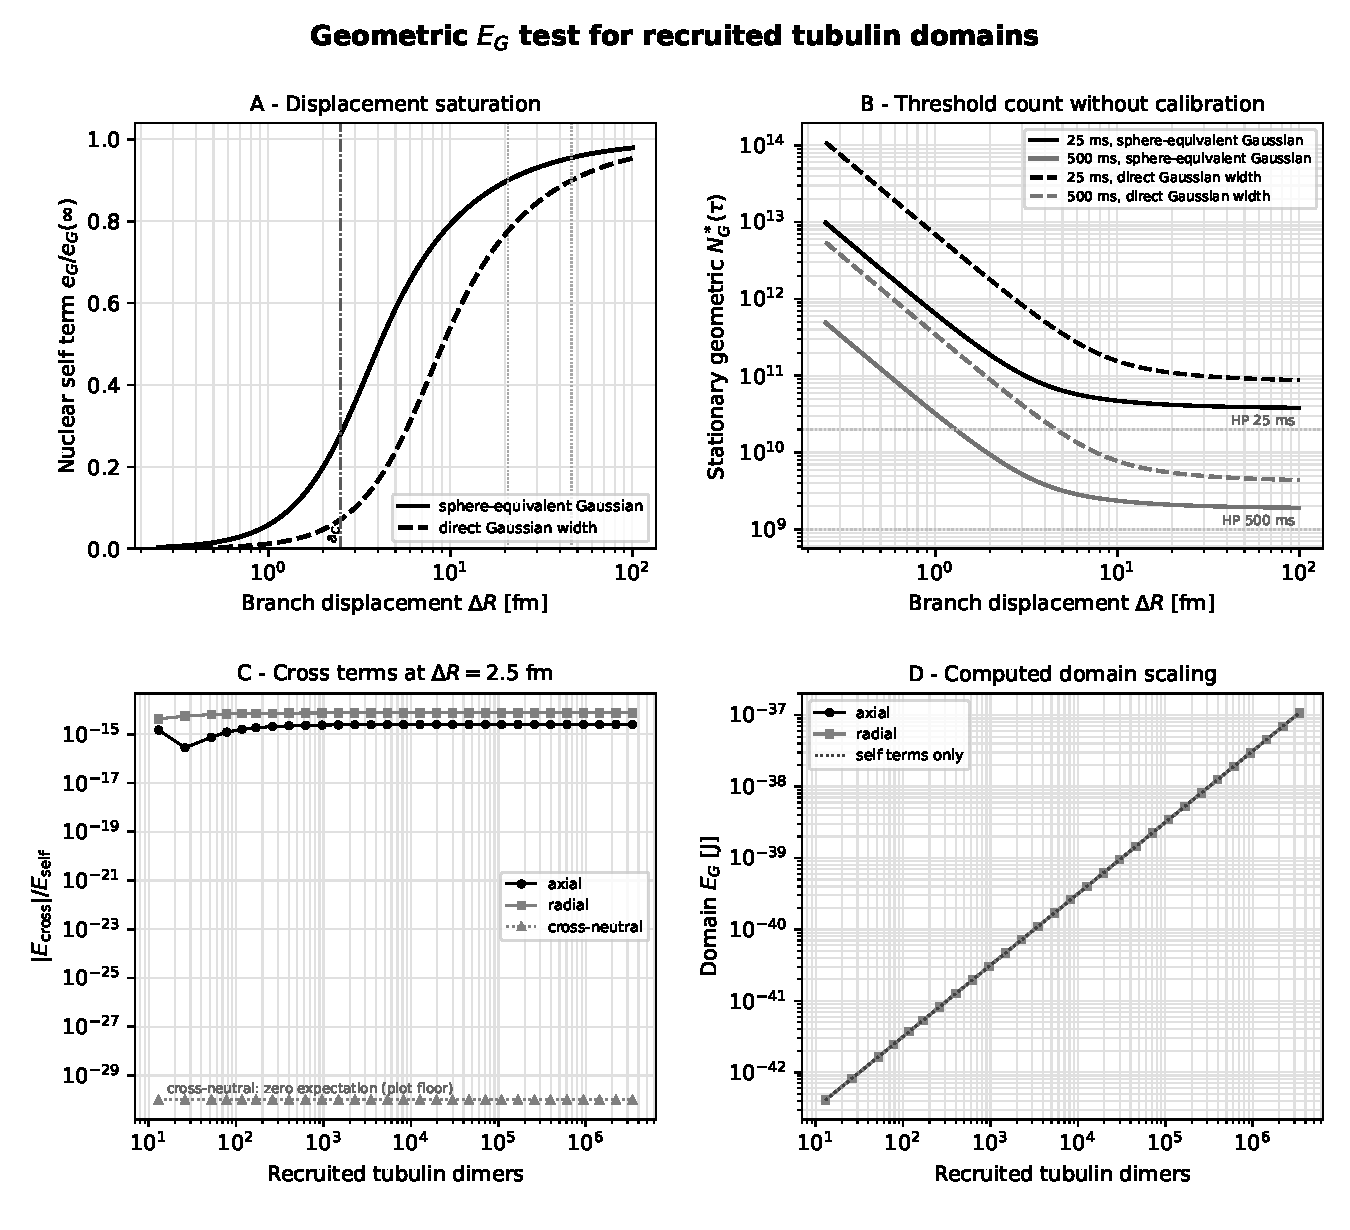
\includegraphics[width=0.94\textwidth]{data/geometric_eg_sweep.pdf}
  \caption{Finite-profile saturation, uncalibrated threshold counts, retained cross
  terms, and domain scaling. At 3,407,872 dimers the axial and radial cross fractions
  are $-2.507\times10^{-15}$ and $+7.535\times10^{-15}$.}
  \label{fig:geometric_eg_sweep}
\end{figure}

\begin{samepage}
\paragraph{Recruitment--reduction lemma.}
For the distributed rigid-displacement geometries evaluated here, write the
single-dimer self term as $e_G(\Delta R,\sigma)$ and the complete domain energy as
\begin{equation}
  E_G(s)=e_G(\Delta R,\sigma)N_i(s)[1+\delta_i(s)],
  \qquad |\delta_i(s)|\leq\varepsilon_{\mathrm{geom}}<1.
  \label{eq:recruitment_reduction_linearisation}
\end{equation}
The numerical sweep gives $\varepsilon_{\mathrm{geom}}<7.6\times10^{-15}$ through
3,407,872 dimers for the tested axial and radial orientations. The pair-Hessian bound
$|\mathbf d_\alpha^{\mathsf T}\nabla\nabla(1/r)\mathbf d_\beta|
\leq2\Delta R^2/r^3$ gives the per-dimer axial lattice remainder beyond $L$ layers:
\begin{equation}
  \left|e_{\mathrm{cross}}^{(\infty)}-e_{\mathrm{cross}}^{(L)}\right|
  \leq
  \frac{2P\,Gm_d^2\Delta R^2}{a_z^3L^2},
  \label{eq:geometric_cross_tail_bound}
\end{equation}
where $P=13$, $a_z=8$ nm, and $m_d=101.93$ kDa. At $L=262144$ and
$\Delta R=2.5$ fm, the bound is $8.84\times10^{-69}$ J per dimer, or
$2.81\times10^{-25}$ of the nuclear self term. For this finite-cross-section
geometry, the lattice contribution therefore has a convergent per-dimer limit and
cannot develop an $N^2$ term as cylinder length increases. The threshold tables give
the total count across recruited domains; cross-domain terms for any specified
arrangement remain governed by Eq.~\eqref{eq:eg} rather than by an assumed scaling
rule. Substitution into
Eq.~\eqref{eq:adaptive_or_trigger} gives
\begin{equation}
  \frac{\hbar}{e_G(1+\varepsilon_{\mathrm{geom}})}
  \leq \int_0^{\tau_i}N_i(s)\,ds
  \leq \frac{\hbar}{e_G(1-\varepsilon_{\mathrm{geom}})},
  \qquad
  \overline N_i=\frac{1}{\tau_i}\int_0^{\tau_i}N_i(s)\,ds.
  \label{eq:recruitment_reduction_bound}
\end{equation}
Reduction therefore depends on accumulated recruitment rather than an
instantaneous carrier count. Different pump trajectories reach the same threshold
when they supply the same integrated load within these geometric bounds.
\end{samepage}

\begin{table}[H]
\centering
\scriptsize
\renewcommand{\arraystretch}{0.88}
\begin{tabular}{@{}
  >{\raggedright\arraybackslash}p{3.2cm}
  >{\raggedright\arraybackslash}p{4.0cm}
  >{\raggedright\arraybackslash}p{5.2cm}@{}}
\toprule
Input & Value and status & Use in the calculation \\
\midrule
Nuclear profile & $a_C\simeq2.5$ fm; few-fm branch displacement; literature model choice \citep{hameroff2014} & Finite branch-density profile in $E_G$; not identified with a stochastic noise length $R_0$. \\
Tubulin geometry & 1JFF alpha--beta dimer; 6,578 modelled heavy atoms and 838/896 deposited residues \citep{lowe2001} & Supplies the independent nuclear coordinates and the completeness correction. \\
Domain geometry & 13 protofilaments, 8 nm axial dimer spacing \citep{fourniol2010} & Supplies the distributed recruitment lattice for the cross-term and domain-size sweep. \\
Profile-width sweep & $\sigma_C=a_C/\sqrt{5}$ and $\sigma_C=a_C$; $\sigma_\nu=\sigma_C(A_\nu/12)^{1/3}$ & Brackets two readings of the 2.5 fm profile input and records the mass-number scaling used for non-carbon nuclei. \\
Electronic separation & order 1 nm; literature model choice \citep{hameroff2014} & Physical route associated by Orch OR with the nuclear-scale displacement. \\
Carrier anchor & $10^9$ tubulins at 500 ms and $2\times10^{10}$ at 25 ms; approximate literature result \citep{hameroff2014} & Fixes $\epsilon_{G,\mathrm{HP}}$ and the conditional $N_{\mathrm{HP}}^*(\tau_i)$ benchmark. \\
Recruitment law & Pump, loss, redistribution, and network coupling \citep{zhang2019frohlich,wang2022frohlich,diazpalencia2025} & Determines $\Omega_i(s)$ and $N_i(s)$ before reduction. \\
Geometric scaling & Full molecular and lattice mass-density calculations \citep{figurato2024,tomaz2024}; Table~\ref{tab:geometric_eg_profiles} & Evaluates self and cross terms on the CDT-induced rest geometry. \\
\bottomrule
\end{tabular}
\caption{Parameter provenance for the geometric $E_G$ and recruitment calculation.}
\label{tab:orch_or_parameter_provenance}
\end{table}

\noindent\begin{minipage}{\linewidth}
\noindent\textit{Stochastic-model comparison.}
LISA Pathfinder gives $\sigma_{\mathrm{DP}}>(40.1\pm0.5)$ fm; Gran Sasso excludes
the natural Markovian version; XENONnT gives $R_0>4.5\times10^{-10}$ m at 95\% CL
\citep{helou2017,donadi2021,xenon2026collapse}. These bounds apply to universal DP
noise dynamics. Their noise lengths are not inputs to the Orch-OR branch calculation.
\end{minipage}

All steps compose into one dependency chain.
\begin{equation}
  \begin{gathered}
  \begin{aligned}
  \hat H|\Phi\rangle=0
  &\longmapsto \rho_Q
  \xrightarrow{\ \operatorname{Tr}(\rho_Q\hat C_\gamma)\ }
  \Gamma_{\mathrm{server}},\\
  \{T\}_{Z_{\mathrm{CDT}}}
  &\xrightarrow{\ \mathcal C_\ell\ }
  (\overline g_{\mu\nu}^{(\ell)},e_\mu^{AA'},u_i^\mu,
   h_{\mu\nu}^{(i)},\mathcal G_{h_i})
  \longmapsto \mathcal L_{\xi_i}^{\mathrm{loc}},\\
  (\Gamma_{\mathrm{server}},\mathcal L_{\xi_i}^{\mathrm{loc}},n)
  &\xrightarrow{\ \Pi_i^{(n)},\ \mathrm{Eq.}\,\eqref{eq:server_relation_read}\ }
  D_i^{\mathrm{server},(n)}.
  \end{aligned}\\[-2pt]
  \underbrace{\begin{aligned}
  (D_i^{\mathrm{local}},D_i^{\mathrm{server}},G_i;u_i)
  &\longmapsto \Gamma_i^{(n)}(\omega_{i\gamma}^{(n)})
  \longmapsto \mathfrak B_i^{(n)}
  \longmapsto |\chi_i(0)\rangle,\\
  |\chi_i(0)\rangle
  &\xrightarrow[\ s_i<\tau_i\ ]{\ Q,\ r^{\mathrm{eff}}/r_c\ }
  (|\chi_i(s_i)\rangle,\Omega_i(s_i),N_i(s_i)),\\
  (|\chi_i(s_i)\rangle,\Omega_i(s_i))
  &\xrightarrow{\ \Delta\rho_i[h_i],\ E_G,\ A_i(\tau_i)=1\ }
  |\chi_i^{\mathrm{fixed}}\rangle,\\
  |\chi_i^{\mathrm{fixed}}\rangle
  &\xrightarrow{\ \mathrm{AdEx/Wilson--Cowan}\ }\Psi_i,\\
  \Psi_i
  &\xrightarrow{\ \mathrm{Eq.}\,\eqref{eq:server_relation_write}\ }
  (B_i^{(n+1)},\mathcal J_i^{(\leq n+1)};
   \gamma_i^{(n)}\in\Gamma_{\mathrm{server}}),\\
  (B_i^{(n+1)},\mathcal J_i^{(\leq n+1)};
   \gamma_i^{(n)}\in\Gamma_{\mathrm{server}})
  &\rightsquigarrow K_i^{(n+1)}\text{ input conditions}.
  \end{aligned}}_{K_i^{(n)}\text{: one conscious mapping cycle}}
  \end{gathered}
  \label{eq:physical_chain}
\end{equation}
\section{Model Tests and Numerical Results}
\label{app:model_tests}

\subsection{Finite local associative load}

With the load $\alpha=P/N$ and the critical value $\alpha_c\simeq0.14$
\citep{amit1985}, the critical number of patterns is
\begin{equation}
  P_{\mathrm{crit}}\simeq\alpha_c N\simeq0.14N.
  \label{eq:hopfield_finite_load}
\end{equation}
\noindent A finite number of units gives a finite critical load,
$N<\infty\Rightarrow P_{\mathrm{crit}}<\infty$.

\subsection{Measured relational convergence}

Let
\begin{equation}
  \operatorname{Rel}\!\left(\Gamma_i^{(n)}\right)=
  \left\{\gamma:(\gamma,\omega_{i\gamma}^{(n)})\in\Gamma_i^{(n)},\ 
  \omega_{i\gamma}^{(n)}>0\right\}
  \label{eq:available_relation_support}
\end{equation}
be the relation support available in the current cycle. For
$\mathcal R_j\subseteq\operatorname{Rel}(\Gamma_i^{(n)})$ and normalisable cycle
weights, define
\begin{equation}
  d_{ij}^{(n)}=
  \frac{\displaystyle\sum_{\gamma\in\mathcal R_j}\omega_{i\gamma}^{(n)}}
       {\displaystyle\sum_{\gamma\in\operatorname{Rel}(\Gamma_i^{(n)})}
         \omega_{i\gamma}^{(n)}}.
  \label{eq:relational_dominance}
\end{equation}
For at least two nonzero-weight relations, let $r_{\gamma\delta}\in[0,1]$ denote
their model-level semantic or causal relation strength. Then
\begin{equation}
  \eta_{ij}^{(n)}=
  \frac{\displaystyle
    \sum_{\substack{\gamma,\delta\in\mathcal R_j\\\gamma\neq\delta}}
      r_{\gamma\delta}\,
      \omega_{i\gamma}^{(n)}\omega_{i\delta}^{(n)}}
       {\displaystyle
    \sum_{\substack{\gamma,\delta\in\mathcal R_j\\\gamma\neq\delta}}
      \omega_{i\gamma}^{(n)}\omega_{i\delta}^{(n)}}.
  \label{eq:relational_coherence}
\end{equation}
Convergence is
\begin{equation}
  C_{ij}^{(n)}=d_{ij}^{(n)}\eta_{ij}^{(n)},
  \qquad
  C_i^{(n)}=\max_j C_{ij}^{(n)}.
  \label{eq:weighted_convergence}
\end{equation}
The definitions give $0\leq d_{ij}^{(n)},\eta_{ij}^{(n)},C_{ij}^{(n)},C_i^{(n)}\leq1$.

The measured centrality of event $\gamma$ is \citep{leechen2022}
\begin{equation}
  r_\gamma=
  \operatorname{Norm}_{\mathrm{narrative}}\!\left(
    \sum_{\delta\neq\gamma}s_{\gamma\delta}
  \right),
  \label{eq:measured_relational_centrality}
\end{equation}
\noindent$s_{\gamma\delta}$ is the measured semantic similarity or independently
judged causal relation used to estimate the model quantity $r_{\gamma\delta}$.

\begin{table}[H]
\centering
\footnotesize
\begin{tabular}{@{}
  >{\raggedright\arraybackslash}p{3.0cm}
  >{\raggedright\arraybackslash}p{5.5cm}
  >{\raggedright\arraybackslash}p{4.2cm}@{}}
\toprule
Source and sample & Measured comparison & Result used here \\
\midrule
\citet{horner2015}, $N=26$ & closed-loop dependency against independent retrieval & $t(25)=2.57$, $p<0.05$; derived $d_z=0.504$ \\
\citet{horner2015}, $N=26$ & open-loop dependency against independent retrieval & $t(25)=1.80$, $p=0.08$; derived $d_z=0.353$ \\
\citet{horner2015}, $N=26$ & closed-loop--open-loop dependency difference & $t(25)=2.77$, $p<0.05$; derived $d_z=0.543$ \\
\citet{horner2015}, $N=26$ & incidental non-target reinstatement & $t(25)=3.40$, $p<0.01$; derived $d_z=0.667$ \\
\citet{leechen2022}, $N=393$ & unique semantic and causal centrality effects on recall & $\beta=0.17$ and $0.44$, both $p<0.001$; logistic mixed models, $\chi^2$ tests \\
\citet{leechen2022}, $N=15$ & high--low centrality hippocampal recall activity & $t(14)=2.71$, $p=0.017$, $d_z=0.70$ \\
\citet{leechen2022}, $N=15$ & high--low semantic-centrality PMC convergence during recall & $\Delta\mathrm{pISC}=0.019$, $p=0.037$; randomisation test \\
\bottomrule
\end{tabular}
\caption{Source-derived relational-convergence benchmark. Horner et al. isolate
network closure at equal relation count; Lee and Chen measure centrality, recall, and
cross-participant neural convergence. The $d_z$ values for Horner et al. are the
direct transformation $t/\sqrt{N}$. Lee and Chen's raw data are archived at
\href{https://doi.org/10.18112/openneuro.ds004042.v1.0.0}{OpenNeuro ds004042}; their
behavioural data and annotations are archived at
\href{https://github.com/jchenlab-jhu/filmfest}{jchenlab-jhu/filmfest}.}
\label{tab:relational_convergence_data}
\end{table}

Because relation structure is measured before recall, this benchmark requires no
model calibration. The prospective comparison and its recorded variables are given in
Table~\ref{tab:relational_convergence_protocol}.

\begin{table}[H]
\centering
\footnotesize
\begin{tabular}{@{}p{3.0cm}p{4.8cm}p{5.3cm}@{}}
\toprule
Protocol element & Specification & Recorded variables \\
\midrule
Shared condition & shared event anchor; complementary person, place, or object relations encoded in one local configuration & isolated retrieval from the other interpreter using the anchor as partial cue \\
Matched condition & same target; no shared event relation & identical retrieval procedure \\
Pre-registration & condition, target, correct response & fixed before measurement \\
Outcomes & forced choice and response process & accuracy, response time, confidence stability, incidental non-target reconstruction, source/perspective errors \\
\bottomrule
\end{tabular}
\caption{Prospective relational-convergence protocol.}
\label{tab:relational_convergence_protocol}
\end{table}

With $B_i(t)$, $H_i$, $G_i$, cue exposure, target, task, and response method matched,
let $j_{\mathrm{target}}$ denote the preregistered target relation set and let
$T_{i,\mathrm{resp}}$ be the measured interval from cue onset to a stable response.
The prospective group-level hypothesis is
\begin{equation}
\begin{aligned}
  \mathbb{E}[C_{i,j_{\mathrm{target}}}\mid\mathrm{shared}]&>
    \mathbb{E}[C_{i,j_{\mathrm{target}}}\mid\mathrm{matched}],\\
  \mathbb{E}[\mathcal F_{i,\mathrm{event}}\mid\mathrm{shared}]&>
    \mathbb{E}[\mathcal F_{i,\mathrm{event}}\mid\mathrm{matched}],\\
  \mathbb{E}[T_{i,\mathrm{resp}}\mid\mathrm{shared}]&<
    \mathbb{E}[T_{i,\mathrm{resp}}\mid\mathrm{matched}].
\end{aligned}
  \label{eq:cross_client_convergence_hypothesis}
\end{equation}
\subsection{Adaptive trigger sensitivity}

For constant input, $w_i=a(V-E_L)$, and the saddle-node rheobase is
\begin{align}
  V_{\mathrm{rheo}}
    &=V_T+\Delta_T\ln\!\left(\frac{g_L+a}{g_L}\right),\\
  I_{\mathrm{rheo}}
    &=(g_L+a)\left[V_T-E_L
      +\Delta_T\ln\!\left(\frac{g_L+a}{g_L}\right)-\Delta_T\right].
  \label{eq:adex_rheobase}
\end{align}
Adaptation is tested over the complete displayed $I/I_{\mathrm{rheo}}$ domain. The two
initial states and numerical controls are given in
Table~\ref{tab:adaptive_trigger_provenance}; their first-spike latencies are shown in
Figure~\ref{fig:adaptive_trigger_sensitivity}.

\begin{table}[H]
\centering
\footnotesize
\begin{tabular}{@{}
  >{\raggedright\arraybackslash}p{3.0cm}
  >{\raggedright\arraybackslash}p{4.0cm}
  >{\raggedright\arraybackslash}p{5.7cm}@{}}
\toprule
Quantity & Value & Status and role \\
\midrule
$C_m,g_L,E_L,$\newline $V_T,\Delta_T$ & 281 pF, 30 nS, $-70.6$ mV, $-50.4$ mV, 2 mV & regular-spiking AdEx source parameters \citep{brettegerstner2005} \\
$\tau_w,a,b$ & 144 ms, 4 nS, 80.5 pA & source parameters defining adaptation \citep{brettegerstner2005} \\
$I_{\mathrm{rheo}}$ & 627.311 pA & derived from Eq.~\eqref{eq:adex_rheobase} \\
$I/I_{\mathrm{rheo}}$ & complete displayed sweep & unknown drive retained as a dimensionless independent variable \\
Integration step & 0.05 ms; checked at 0.025 ms & numerical control; maximum latency change 0.1 ms \\
\bottomrule
\end{tabular}
\caption{Parameter provenance for the adaptive-trigger calculation.}
\label{tab:adaptive_trigger_provenance}
\end{table}

\begin{figure}[ht]
  \centering
  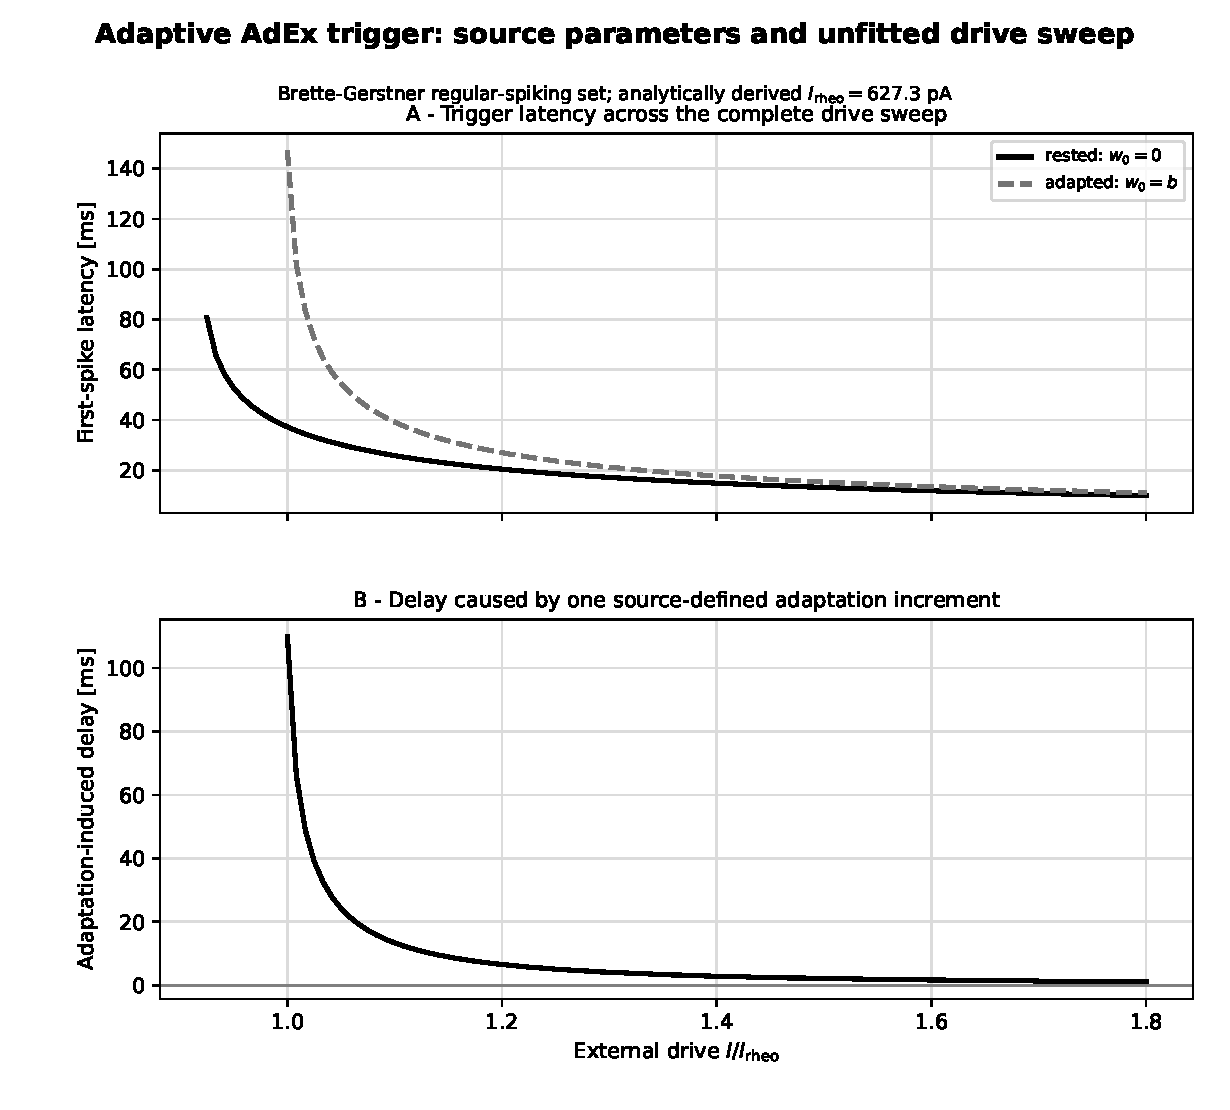
\includegraphics[width=\textwidth]{data/adaptive_trigger_sensitivity.pdf}
  \caption{AdEx trigger sensitivity. The source-defined adaptation increment changes
  first-spike latency across the source-parameterised drive sweep.}
  \label{fig:adaptive_trigger_sensitivity}
\end{figure}

\section{Mapping Disruption and Resynchronisation}
\label{app:mapping_disruption}

The gap is taken between the last stable local state at $t_0^-$ and the first
recovered state at $t_1^+$.
\begin{equation}
  G_i=\operatorname{Gap}\!\left(
    D_i^{\mathrm{local}}(t_0^-),D_i^{\mathrm{local}}(t_1^+)
  \right).
  \label{eq:mapping_gap}
\end{equation}
Resynchronisation repeats the complete mapping cycle.
\begin{align}
  \Psi_i^{(n)}
    &=K_i\!\left(
        D_i^{\mathrm{local},(n)},D_i^{\mathrm{server},(n)},G_i^{(n)}
        \mid u_i
      \right),
      \label{eq:resynchronisation_map}\\
  G_i^{(n+1)}&\subseteq G_i^{(n)},
  \qquad
  G_i^{(n+1)}=\varnothing
  \quad\text{when resynchronisation completes}.
  \label{eq:residual_mapping_gap}
\end{align}
\noindent Here $G_i^{(n+1)}$ is the unresolved remainder passed to the next cycle,
and $\mathcal F_i$ is the fidelity of source, perspective, event, and time.
Inscription follows Eqs.~\eqref{eq:physical_chain}
and~\eqref{eq:server_relation_write}.


% -----------------------------------------------------------------------
% AI-use disclosure. Stand 19.11.2026 (Zenodo-Fassung): heavily AI-assisted.
% Introduction and Sections 2-3 were revised by the author by hand; the wording
% from Section 4 onwards and of the appendices was formulated with AI assistance.
% -----------------------------------------------------------------------
\section*{Use of AI-Assisted Tools}
\noindent This work was heavily AI-assisted. The idea, the model and its central
hypotheses, the way its parts are put together, the line of argument, and all
conclusions are the author's own. The Introduction and
Sections~\ref{sec:existing_models} and~\ref{sec:local_client} were revised by the
author by hand. AI assistance was used for the wording of the text from
Section~\ref{sec:server} onwards and of the appendices, and for typesetting,
simulation, and checking (sources and mathematics). It did not originate the ideas or
the scientific insight.

\bibliographystyle{apalike}
\begingroup
\small
\singlespacing
\sloppy
\setlength{\emergencystretch}{4em}
\setlength{\bibsep}{3pt plus 0.5pt minus 0.5pt}
\setlength{\bibhang}{1.25em}
\bibliography{references}
\endgroup
% M&M: citations by author and year, references listed alphabetically; apalike approximates this.

\end{document}
